\documentclass[aspectratio=169]{beamer}
\setbeamertemplate{navigation symbols}{}
\usepackage{color,amsmath,comment, subfigure}
\usepackage{booktabs}



%%%%%%%%%%%%%%%%%%%%%%%%%%
\title[]{Lecture 20: Social media and social ads}
\author[]{Matthew J. Salganik}
\institute[]{Sociology 204: Social Networks\\Princeton University}
\date[]{
2/2: Social in the ad not just the targeting
\vfill

\begin{flushleft}
\vspace{0.6in}

\includegraphics[width=0.1\textwidth]{figures/cc.png}
\end{flushleft}
}

\begin{document}
%%%%%%%%%%%%%%%%%%%%%%%%%%%
\frame{\titlepage}
%%%%%%%%%%%%%%%%%%%%%%%%%%%
\begin{frame}

"We regard social advertising as any advertising methods that uses information about consumers' social networks to target ads and/or provide personalized social signals.'' Bakshy et al.\

\end{frame}
%%%%%%%%%%%%%%%%%%%
\begin{frame}

\begin{center}
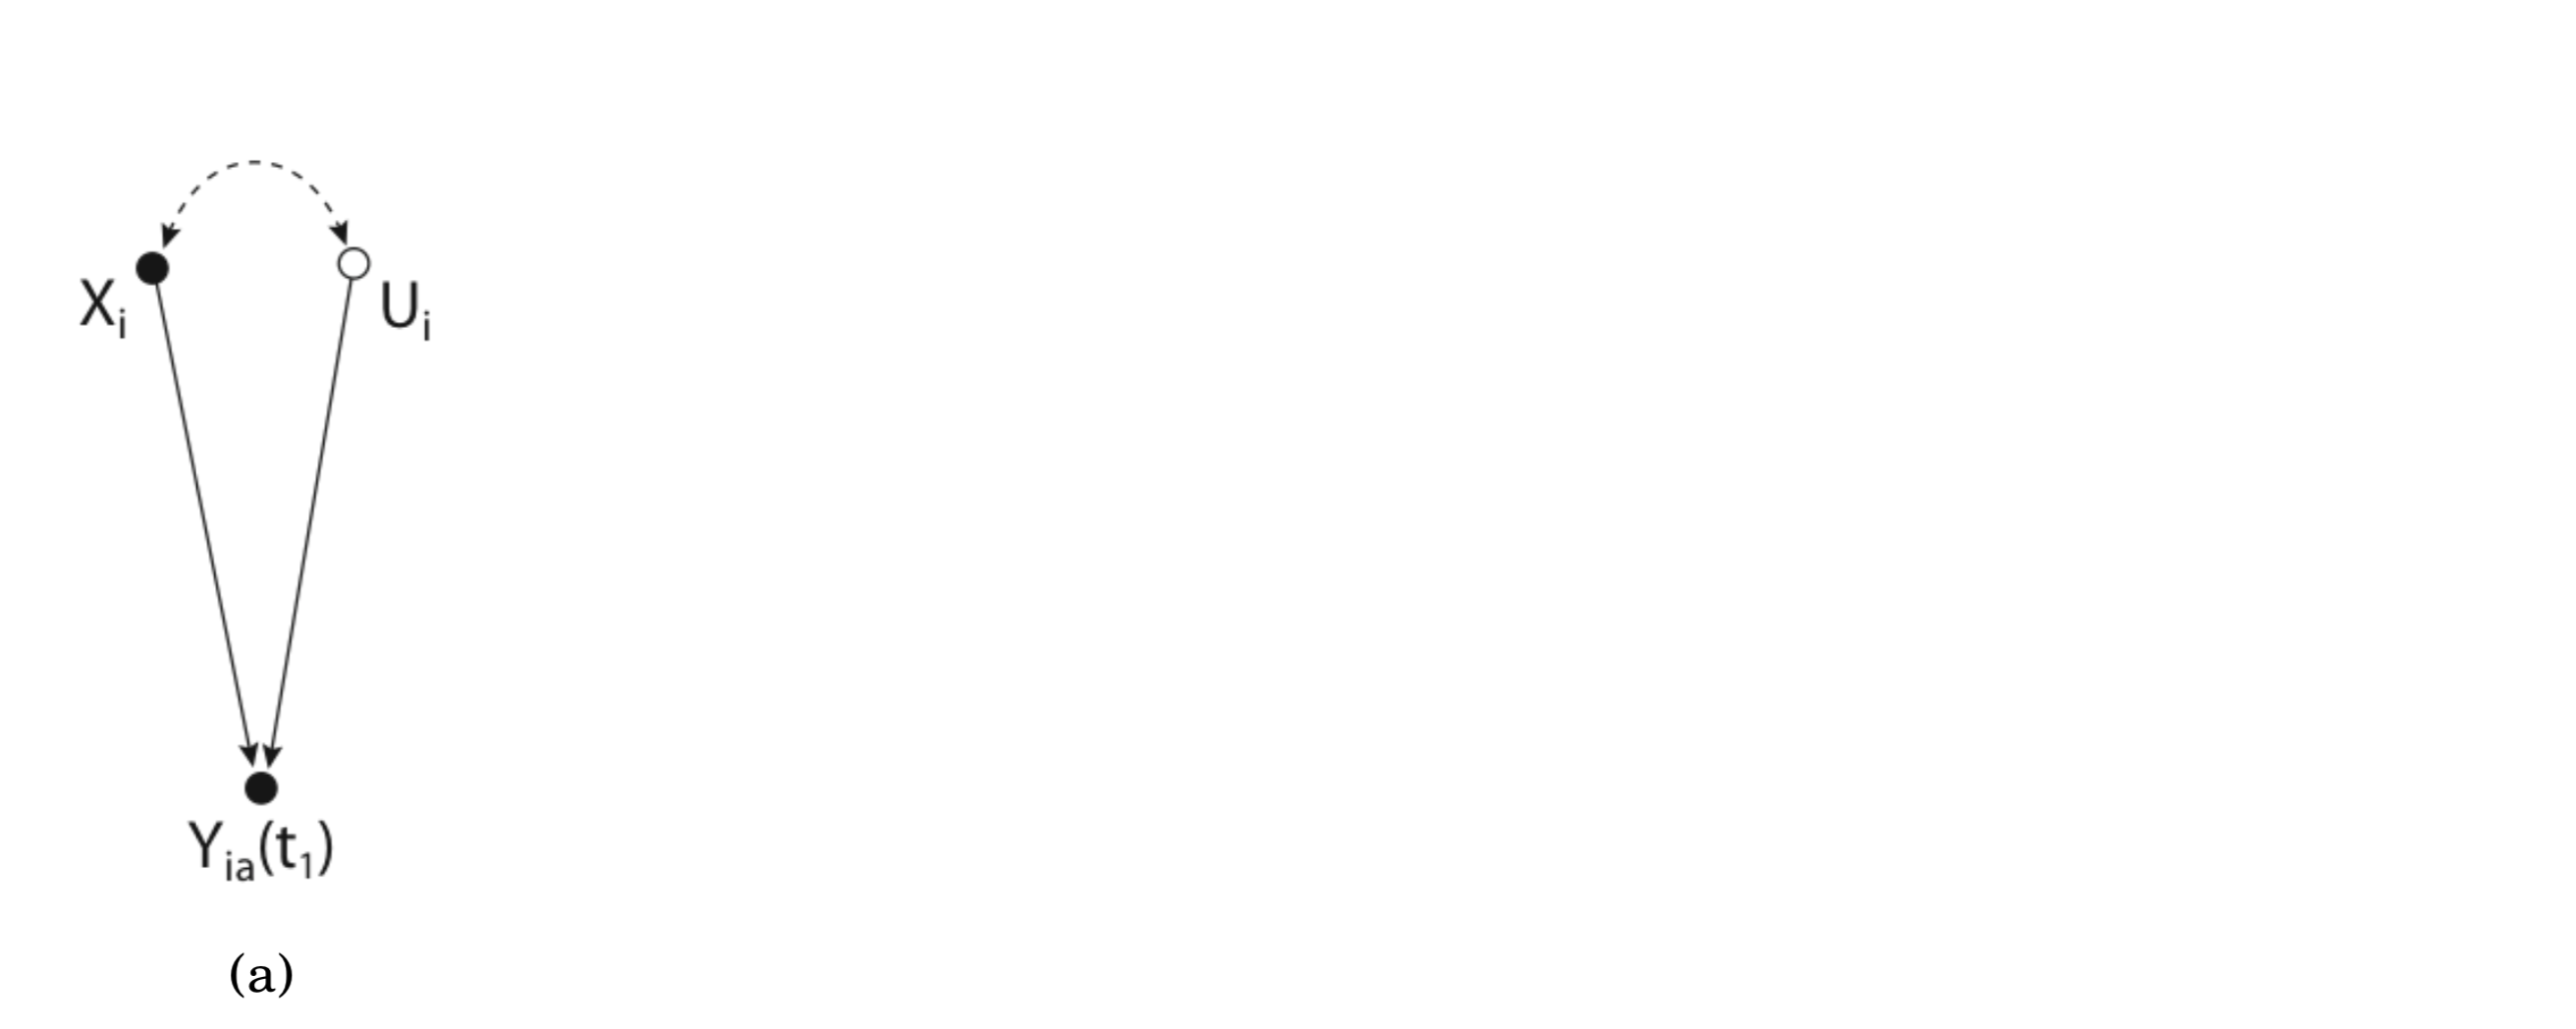
\includegraphics[width=0.8\textwidth]{figures/bakshy_social_2012_fig1a}
\end{center}

\begin{itemize}
\item $Y_{ia}(t_1)$ (person $i$ clicking on ad $a$ at time 1) is caused by measured characteristics $X_i$ and unmeasured characteristics $U_i$.
\item Measured characteristics $X_i$ and unmeasured characteristics $U_i$ might be correlated in unknown ways.
\end{itemize}

\end{frame}
%%%%%%%%%%%%%%%%%
\begin{frame}

\begin{center}
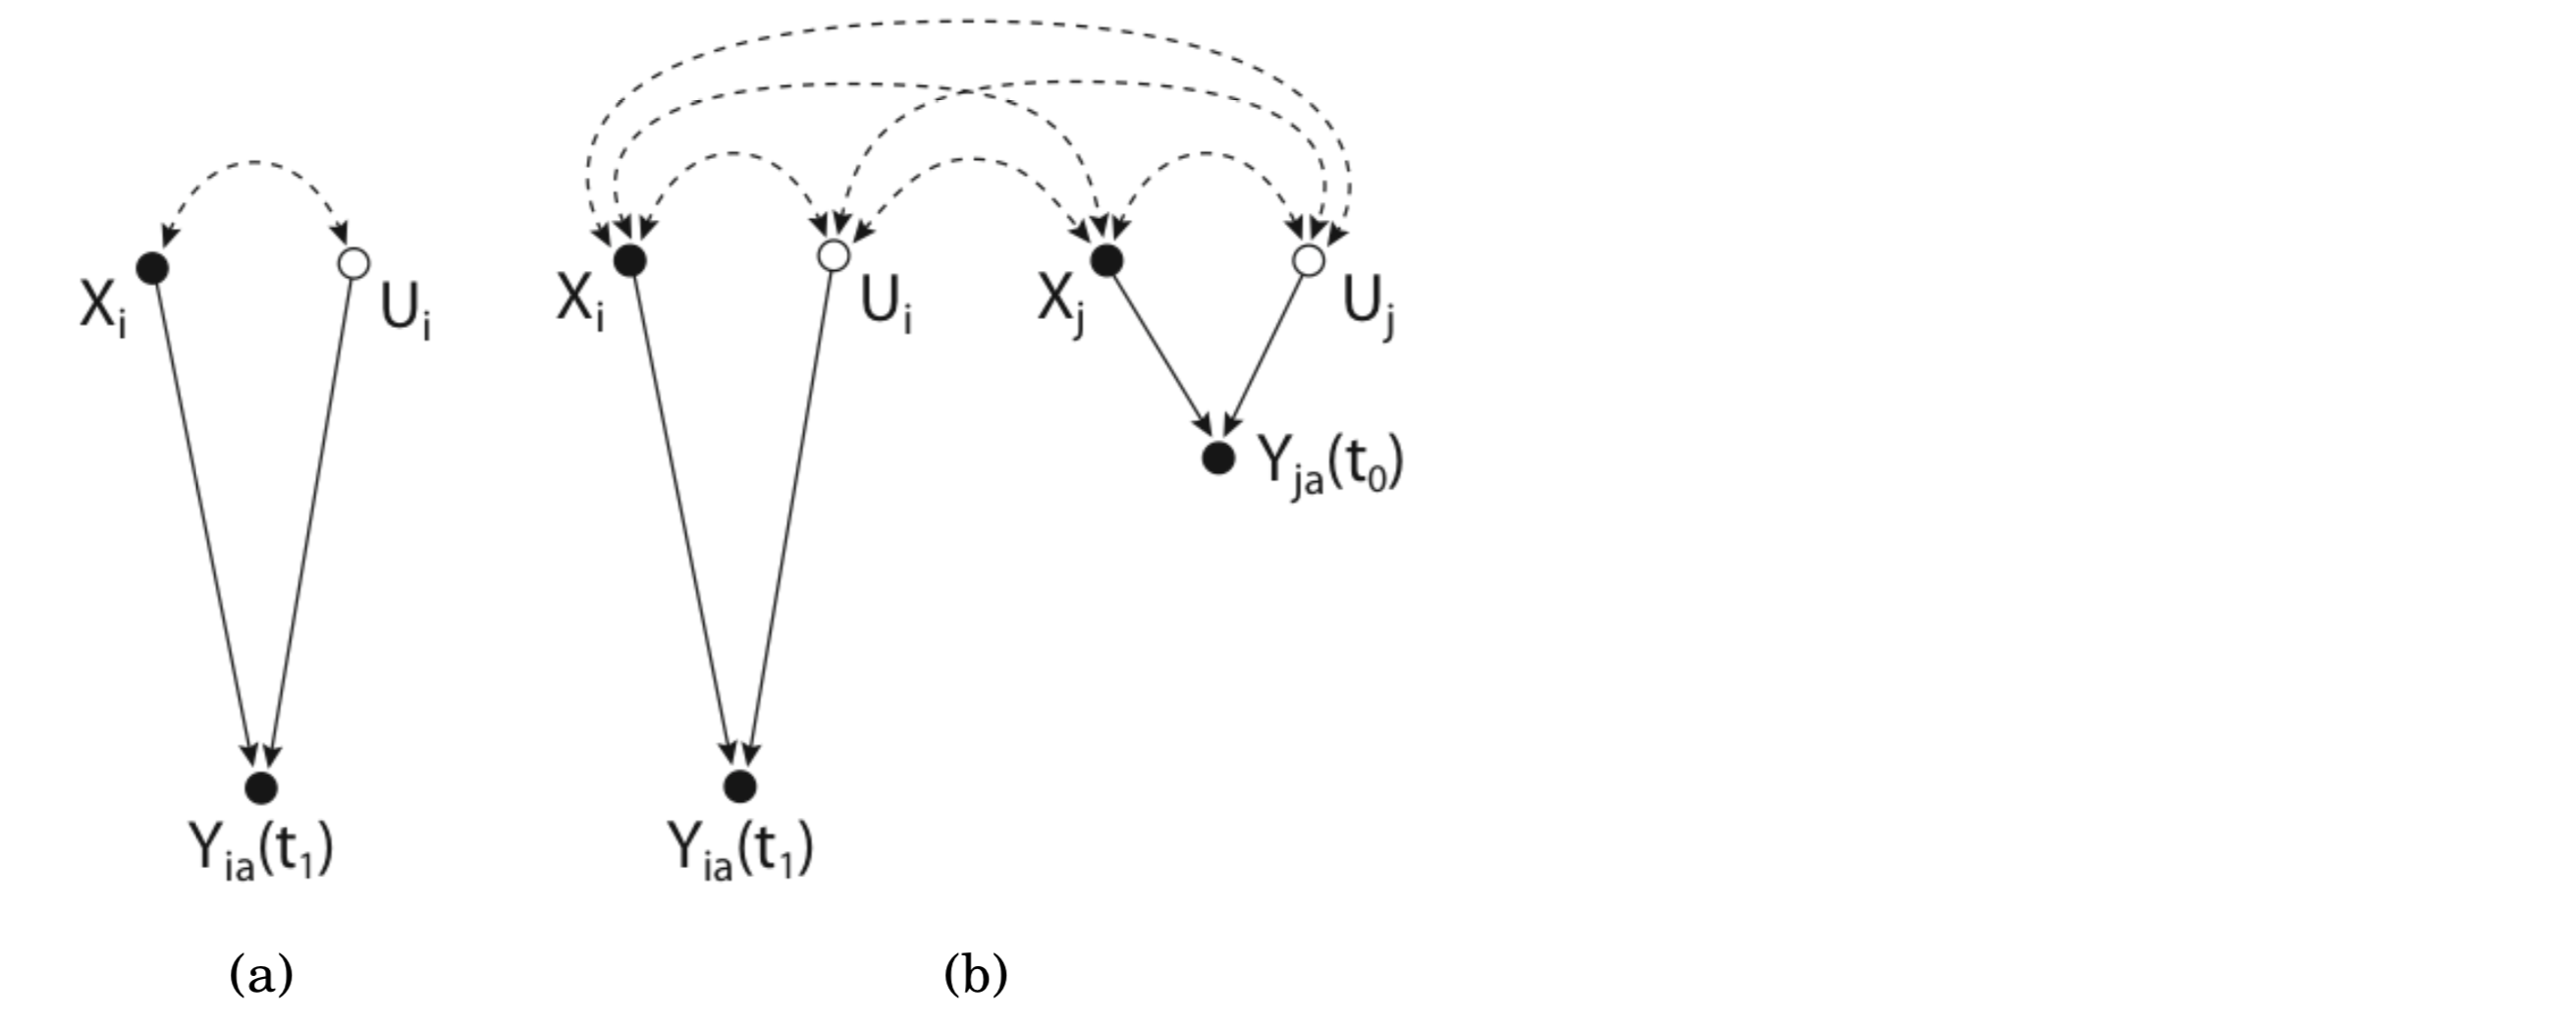
\includegraphics[width=0.6\textwidth]{figures/bakshy_social_2012_fig1ab}
\end{center}

\begin{itemize}
\item $Y_{ia}(t_1)$ (person $i$ clicking on ad $a$ at time 1) is caused by measured characteristics $X_i$ and unmeasured characteristics $U_i$. \pause
\item $Y_{ja}(t_0)$ (person $j$ clicking on ad $a$ at time 0) is caused by measured characteristics $X_j$ and unmeasured characteristics $U_j$. \pause
\item Measured characteristics $X_i$ and $X_j$ and unmeasured characteristics $U_i$ and $U_j$ might be correlated in unknown ways.
\end{itemize}

When there is homophily $j$'s behavior at time $0$ predicts $i$'s behavior at time $1$.

\note{
Example my brother clicks on mini-van ad, I'm more likely. It is like his behavior reveals something bout my unmeasured characteristics.
}

\end{frame}
%%%%%%%%%%%%%%%%%
\begin{frame}

\begin{center}
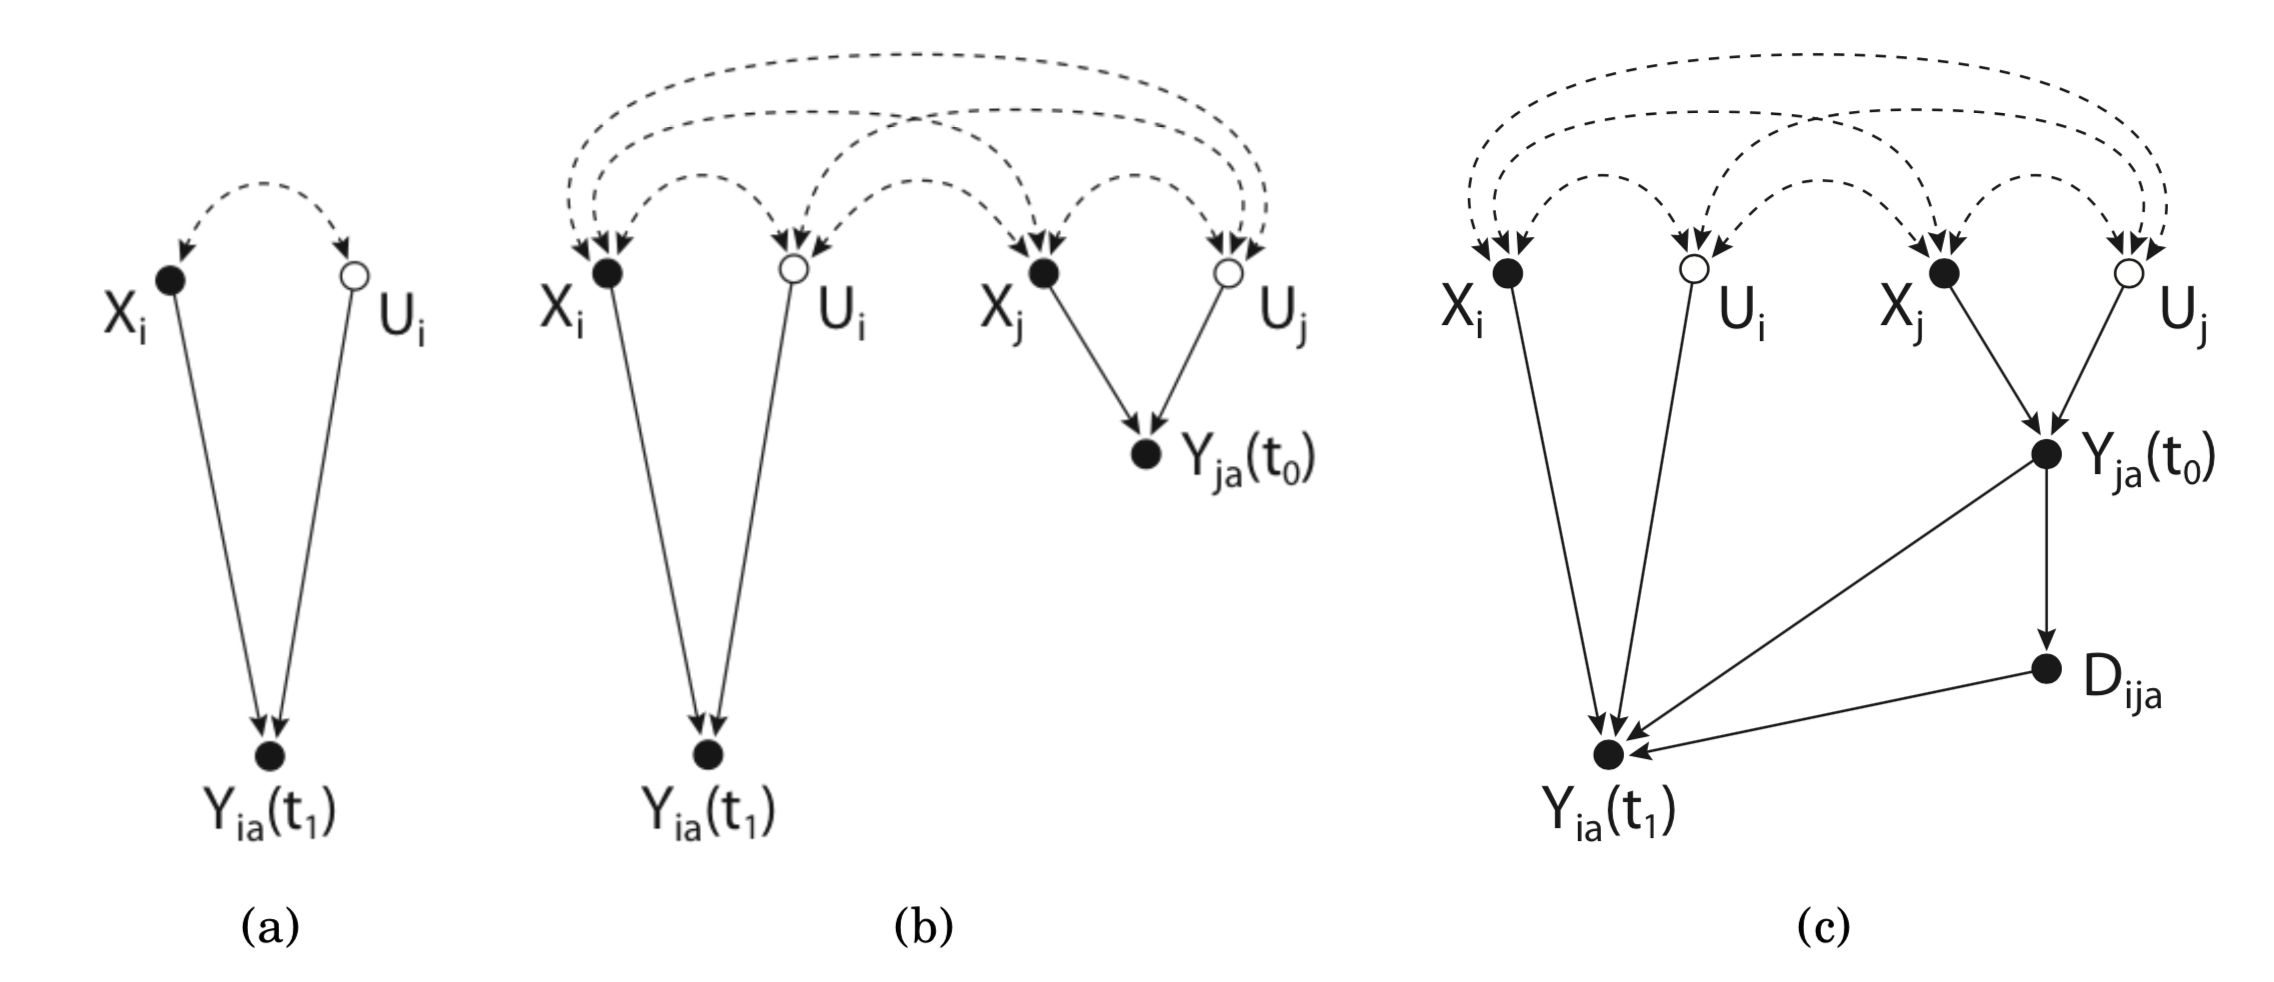
\includegraphics[width=0.6\textwidth]{figures/bakshy_social_2012_fig1}
\end{center}

\begin{itemize}
\item $Y_{ia}(t_1)$ (person $i$ clicking on ad $a$ at time 1) is caused by measured characteristics $X_i$ and unmeasured characteristics $U_i$. \pause
\item $Y_{ja}(t_0)$ (person $j$ clicking on ad $a$ at time 0) is caused by measured characteristics $X_j$ and unmeasured characteristics $U_j$. \pause
\item Measured characteristics $X_i$ and $X_j$ and unmeasured characteristics $U_i$ and $U_j$ might be correlated in unknown ways. \pause
\item Most important new addition: social signal $D_{ija}$ might impact $Y_{ia}(t_1)$.
\end{itemize}

If you see correlated behavior what is causing that?  Social influence or correlation of unmeasured characteristics?

\end{frame}
%%%%%%%%%%%%%%%%
\begin{frame}

\begin{center}
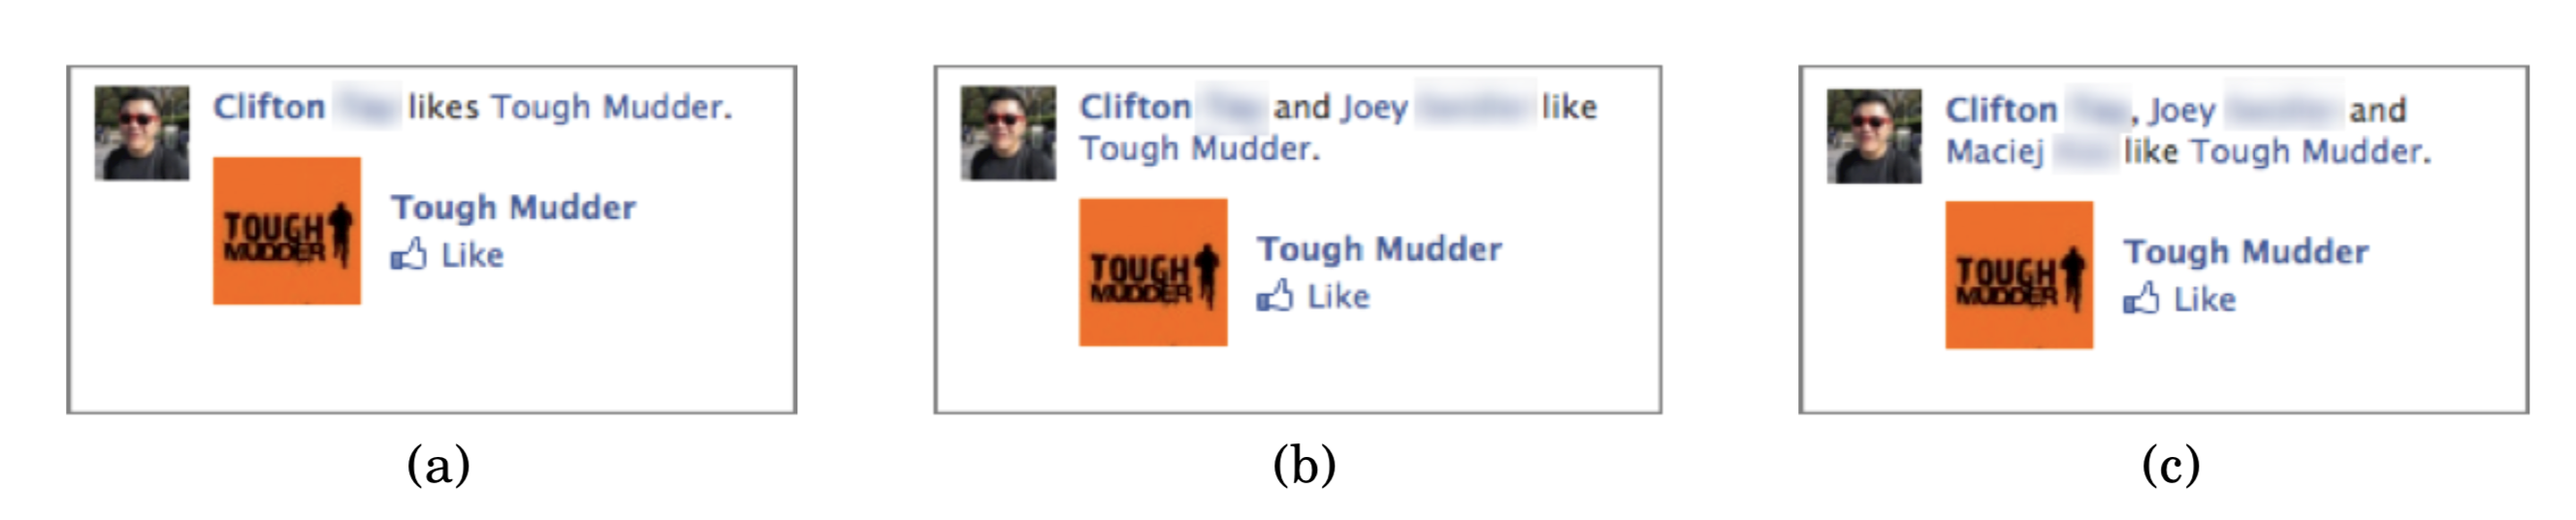
\includegraphics[width=\textwidth]{figures/bakshy_social_2012_fig2}
\end{center}

\end{frame}
%%%%%%%%%%%%%%%%%
\begin{frame}

\begin{center}
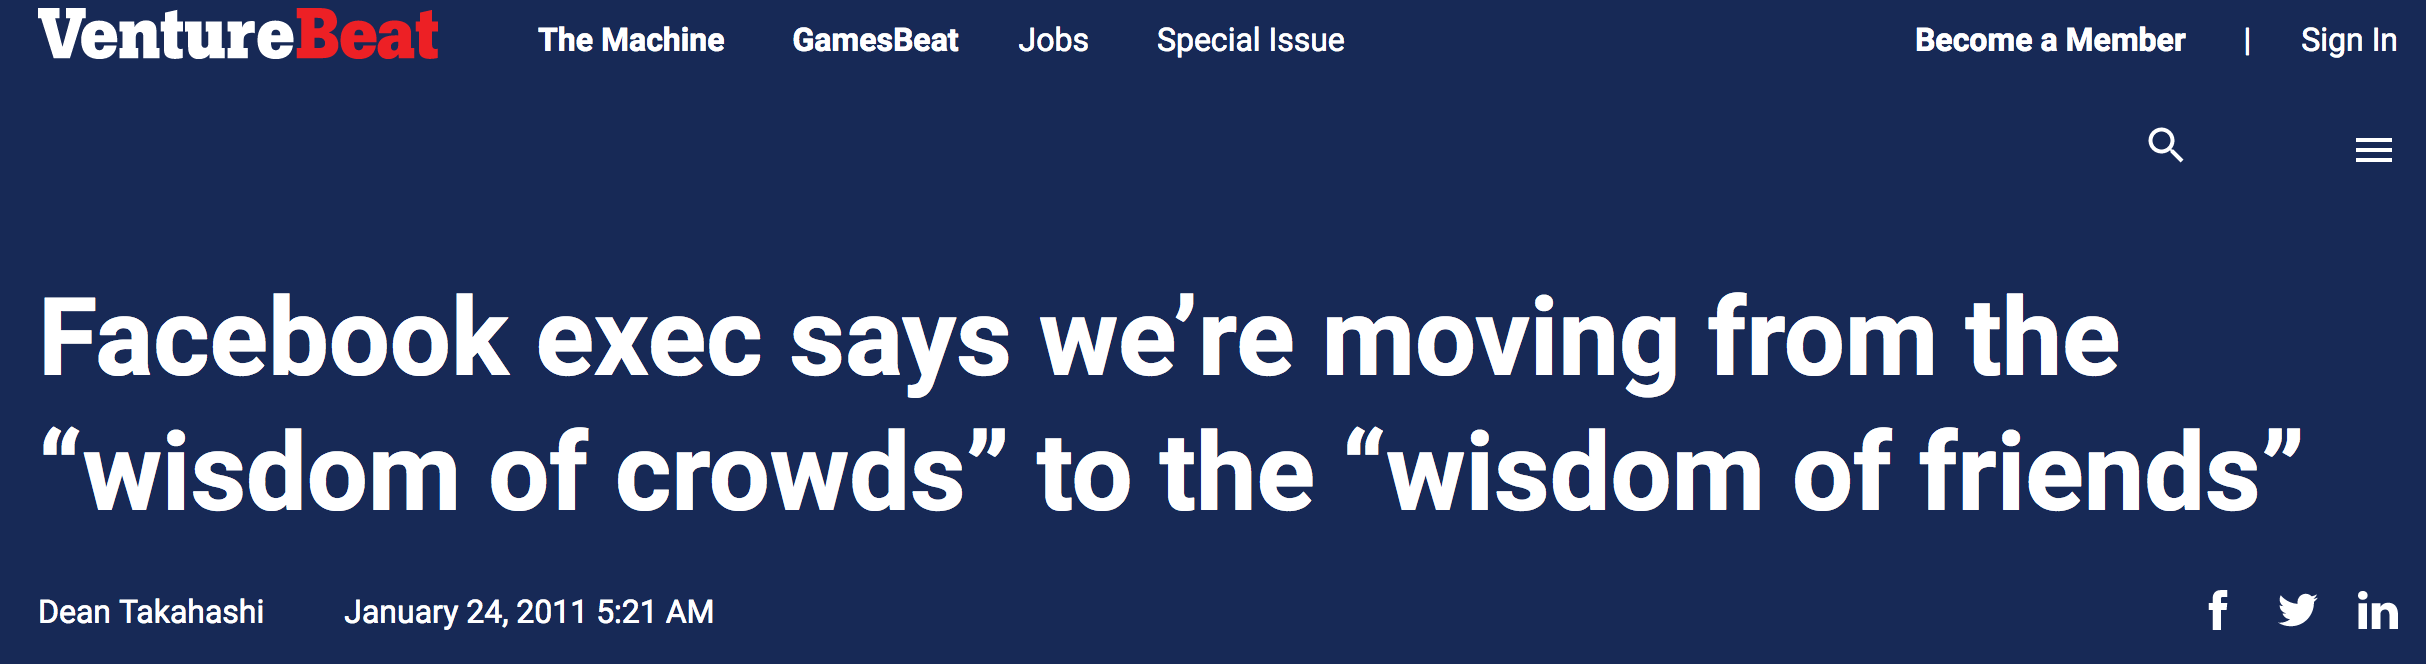
\includegraphics[width=\textwidth]{figures/takahashi_facebook_2011_title}
\end{center}

\vfill
\begin{center}
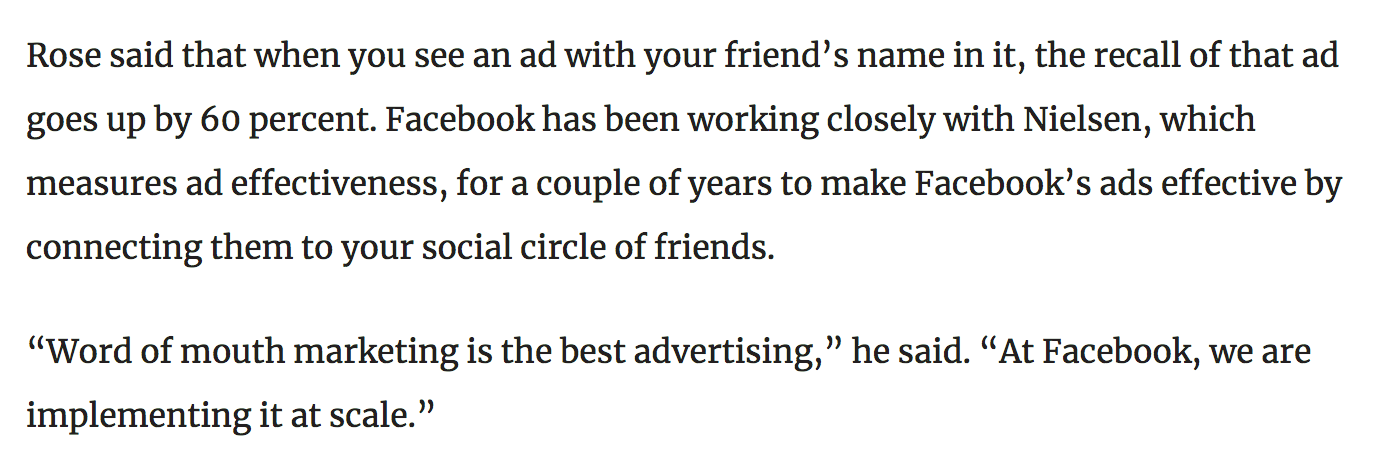
\includegraphics[width=0.8\textwidth]{figures/takahashi_facebook_2011_pullquote}
\end{center}

\end{frame}
%%%%%%%%%%%%%%%%
\begin{frame}

\begin{center}
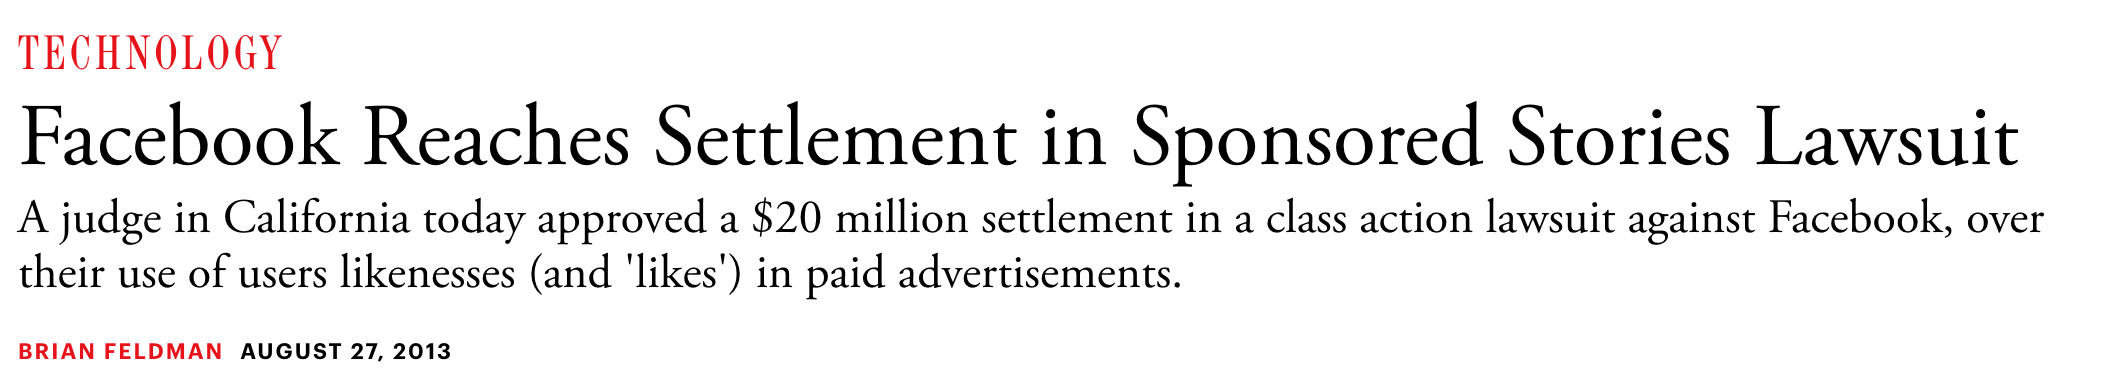
\includegraphics[width=\textwidth]{figures/feldman_facebook_2013_headline}
\end{center}

\vfill
\url{https://www.theatlantic.com/technology/archive/2013/08/facebook-reaches-settlement-sponsored-stories/311753/}
\end{frame}
%%%%%%%%%%%%%%%%%
\begin{frame}

\begin{center}
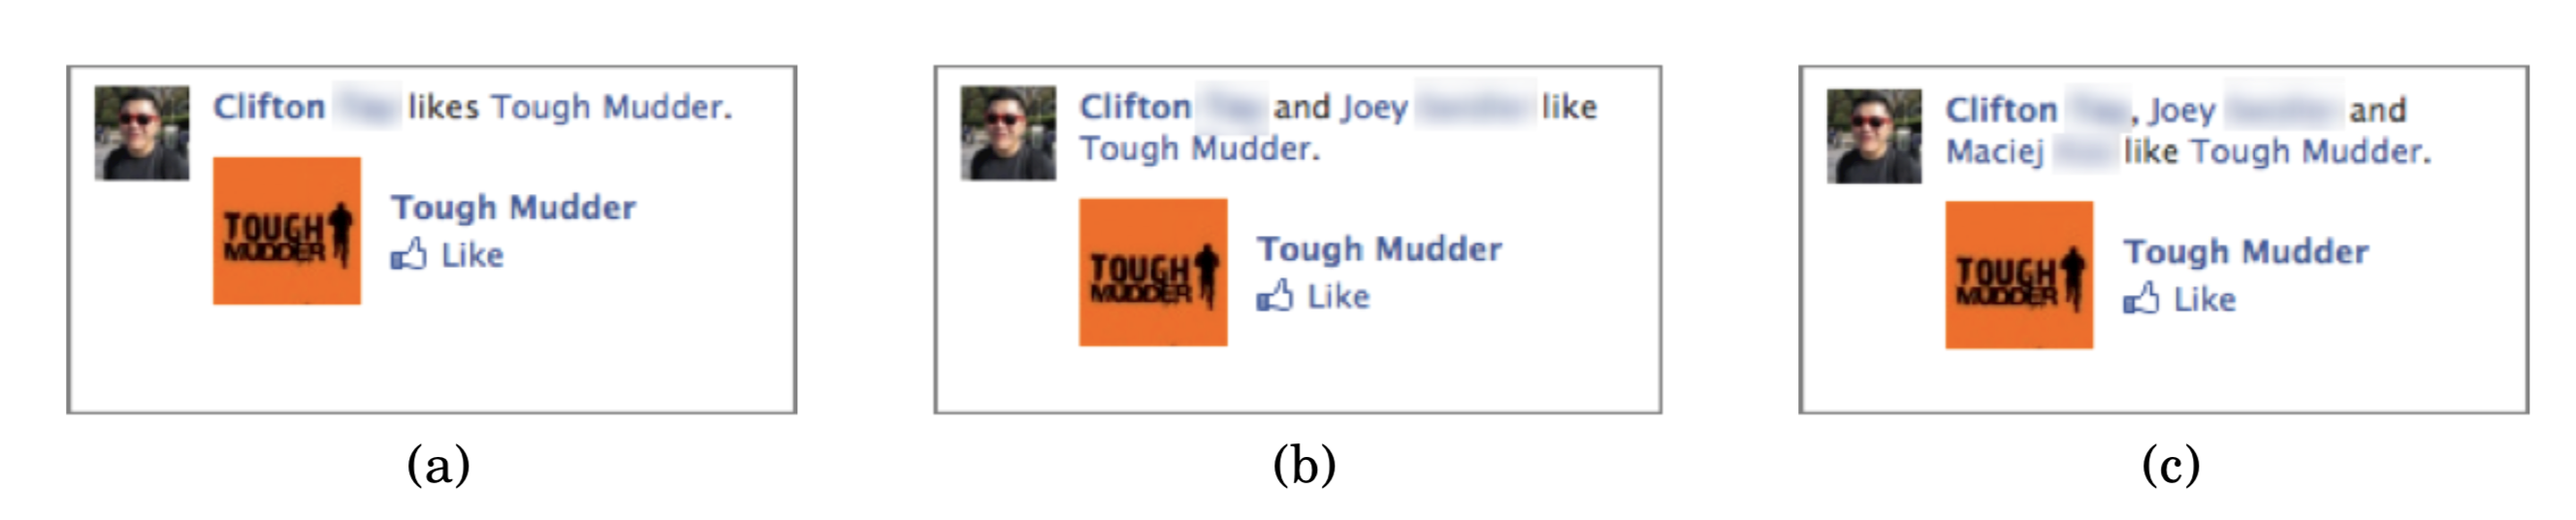
\includegraphics[width=\textwidth]{figures/bakshy_social_2012_fig2}
\end{center}

\end{frame}
%%%%%%%%%%%%%%%%%
\begin{frame}

\begin{figure}
\includegraphics[width=0.75\textwidth]{figures_book/7_1}
\end{figure}

\end{frame}
%%%%%%%%%%%%%%%%%
\begin{frame}

\begin{center}
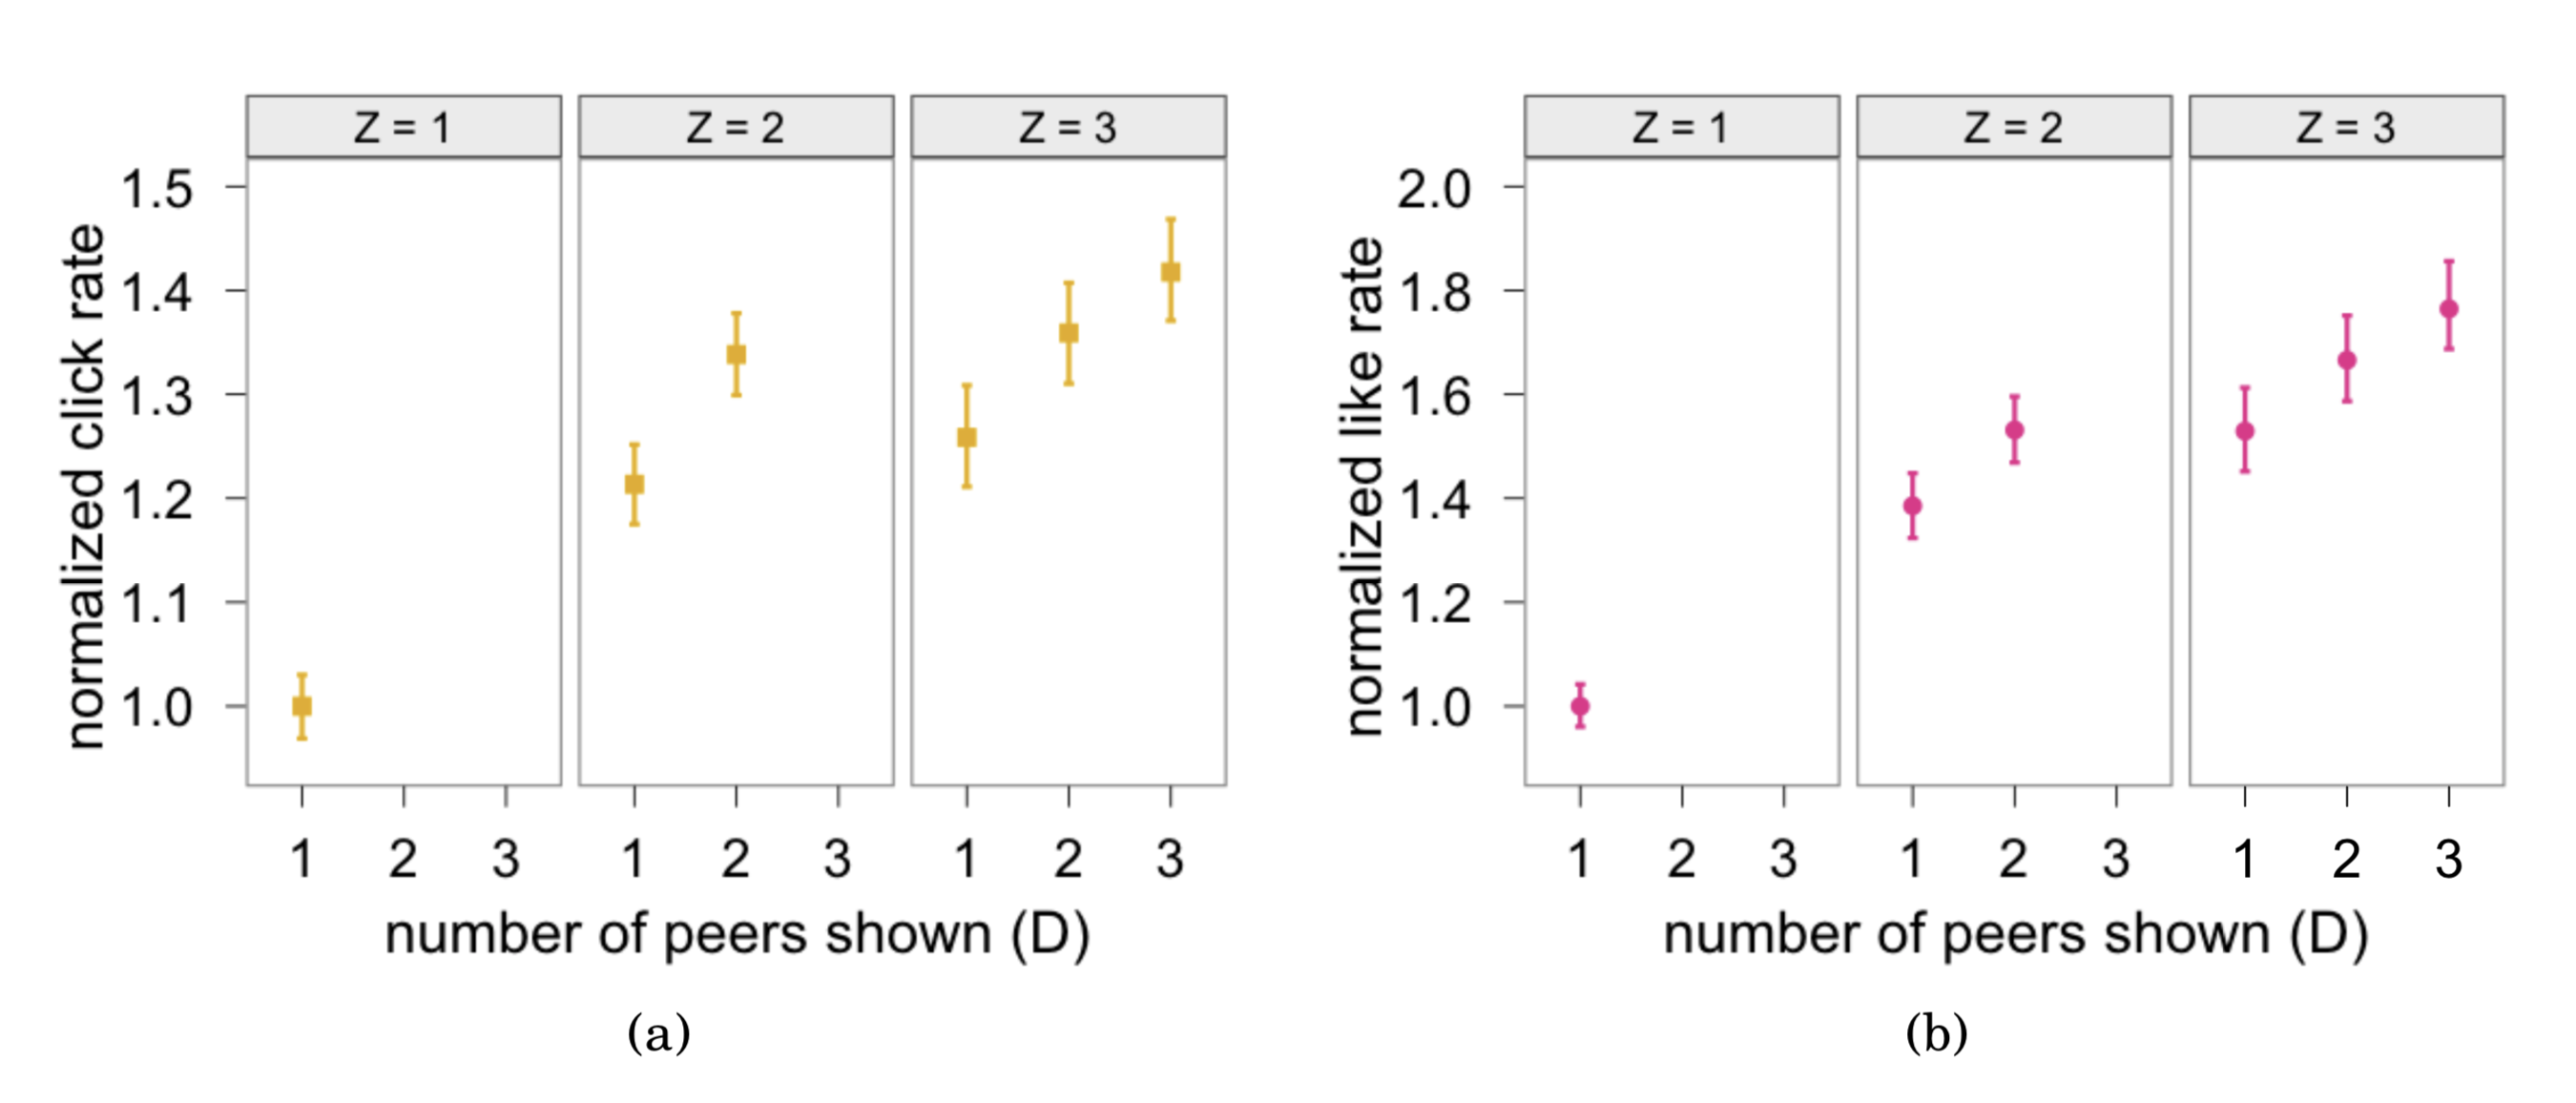
\includegraphics[width=\textwidth]{figures/bakshy_social_2012_fig3}
\end{center}

\vfill
\begin{itemize}
\item For each value of $Z$, more peers shown more clicks and likes
\item Difference between $D=1$ for different values of $Z$ suggests homophily on unobservable characteristics (but with caution)
\item They don't publish raw rates, and papers often go through business review before sending them to a journal
\end{itemize}

\note{
Consistency across two metrics is good to see
}

\end{frame}
%%%%%%%%%%%%%%%%%
\begin{frame}

Experiment 2:
\begin{center}
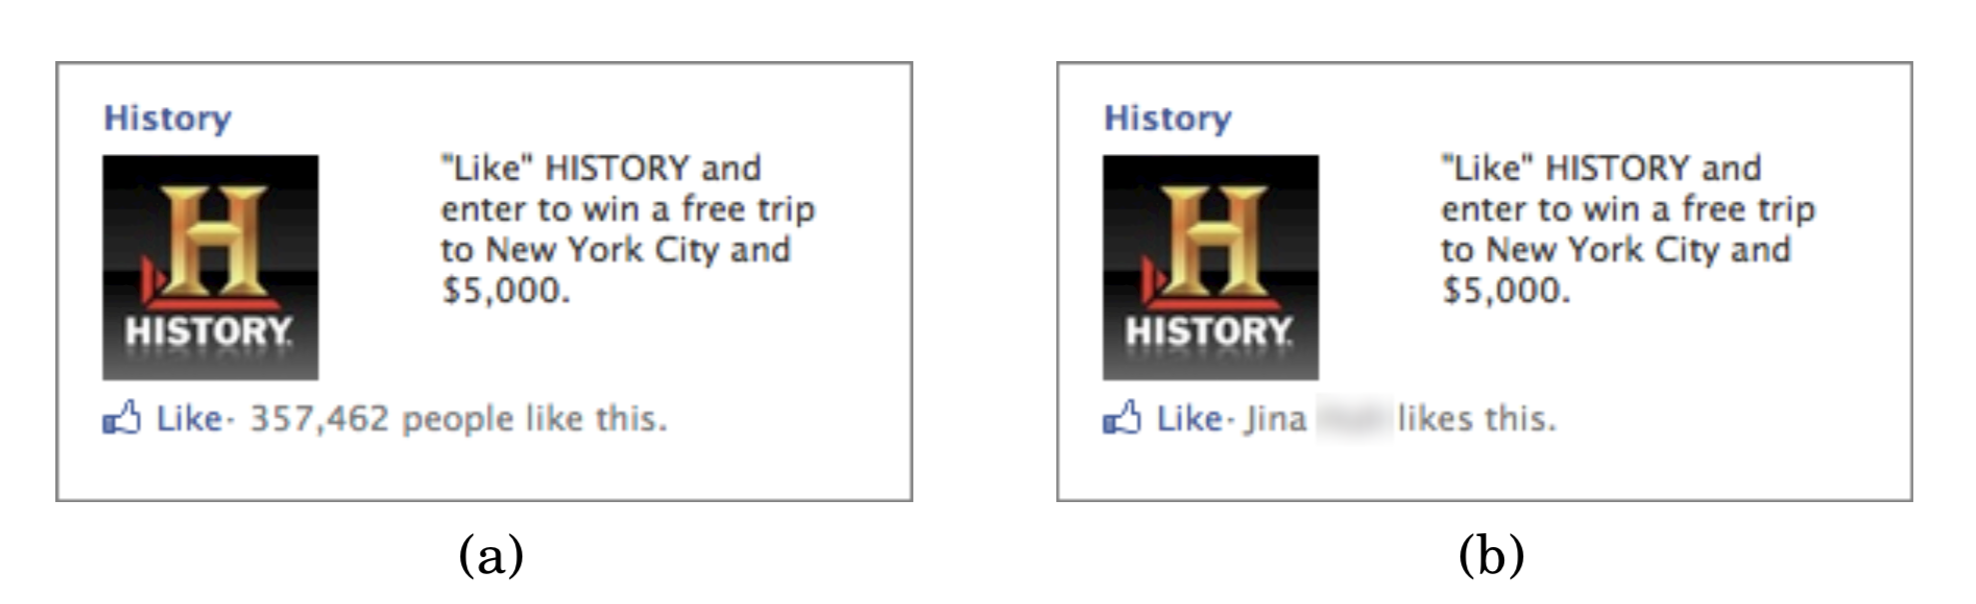
\includegraphics[width=\textwidth]{figures/bakshy_social_2012_fig4}
\end{center}

\end{frame}
%%%%%%%%%%%%%%%%%
\begin{frame}

\begin{center}
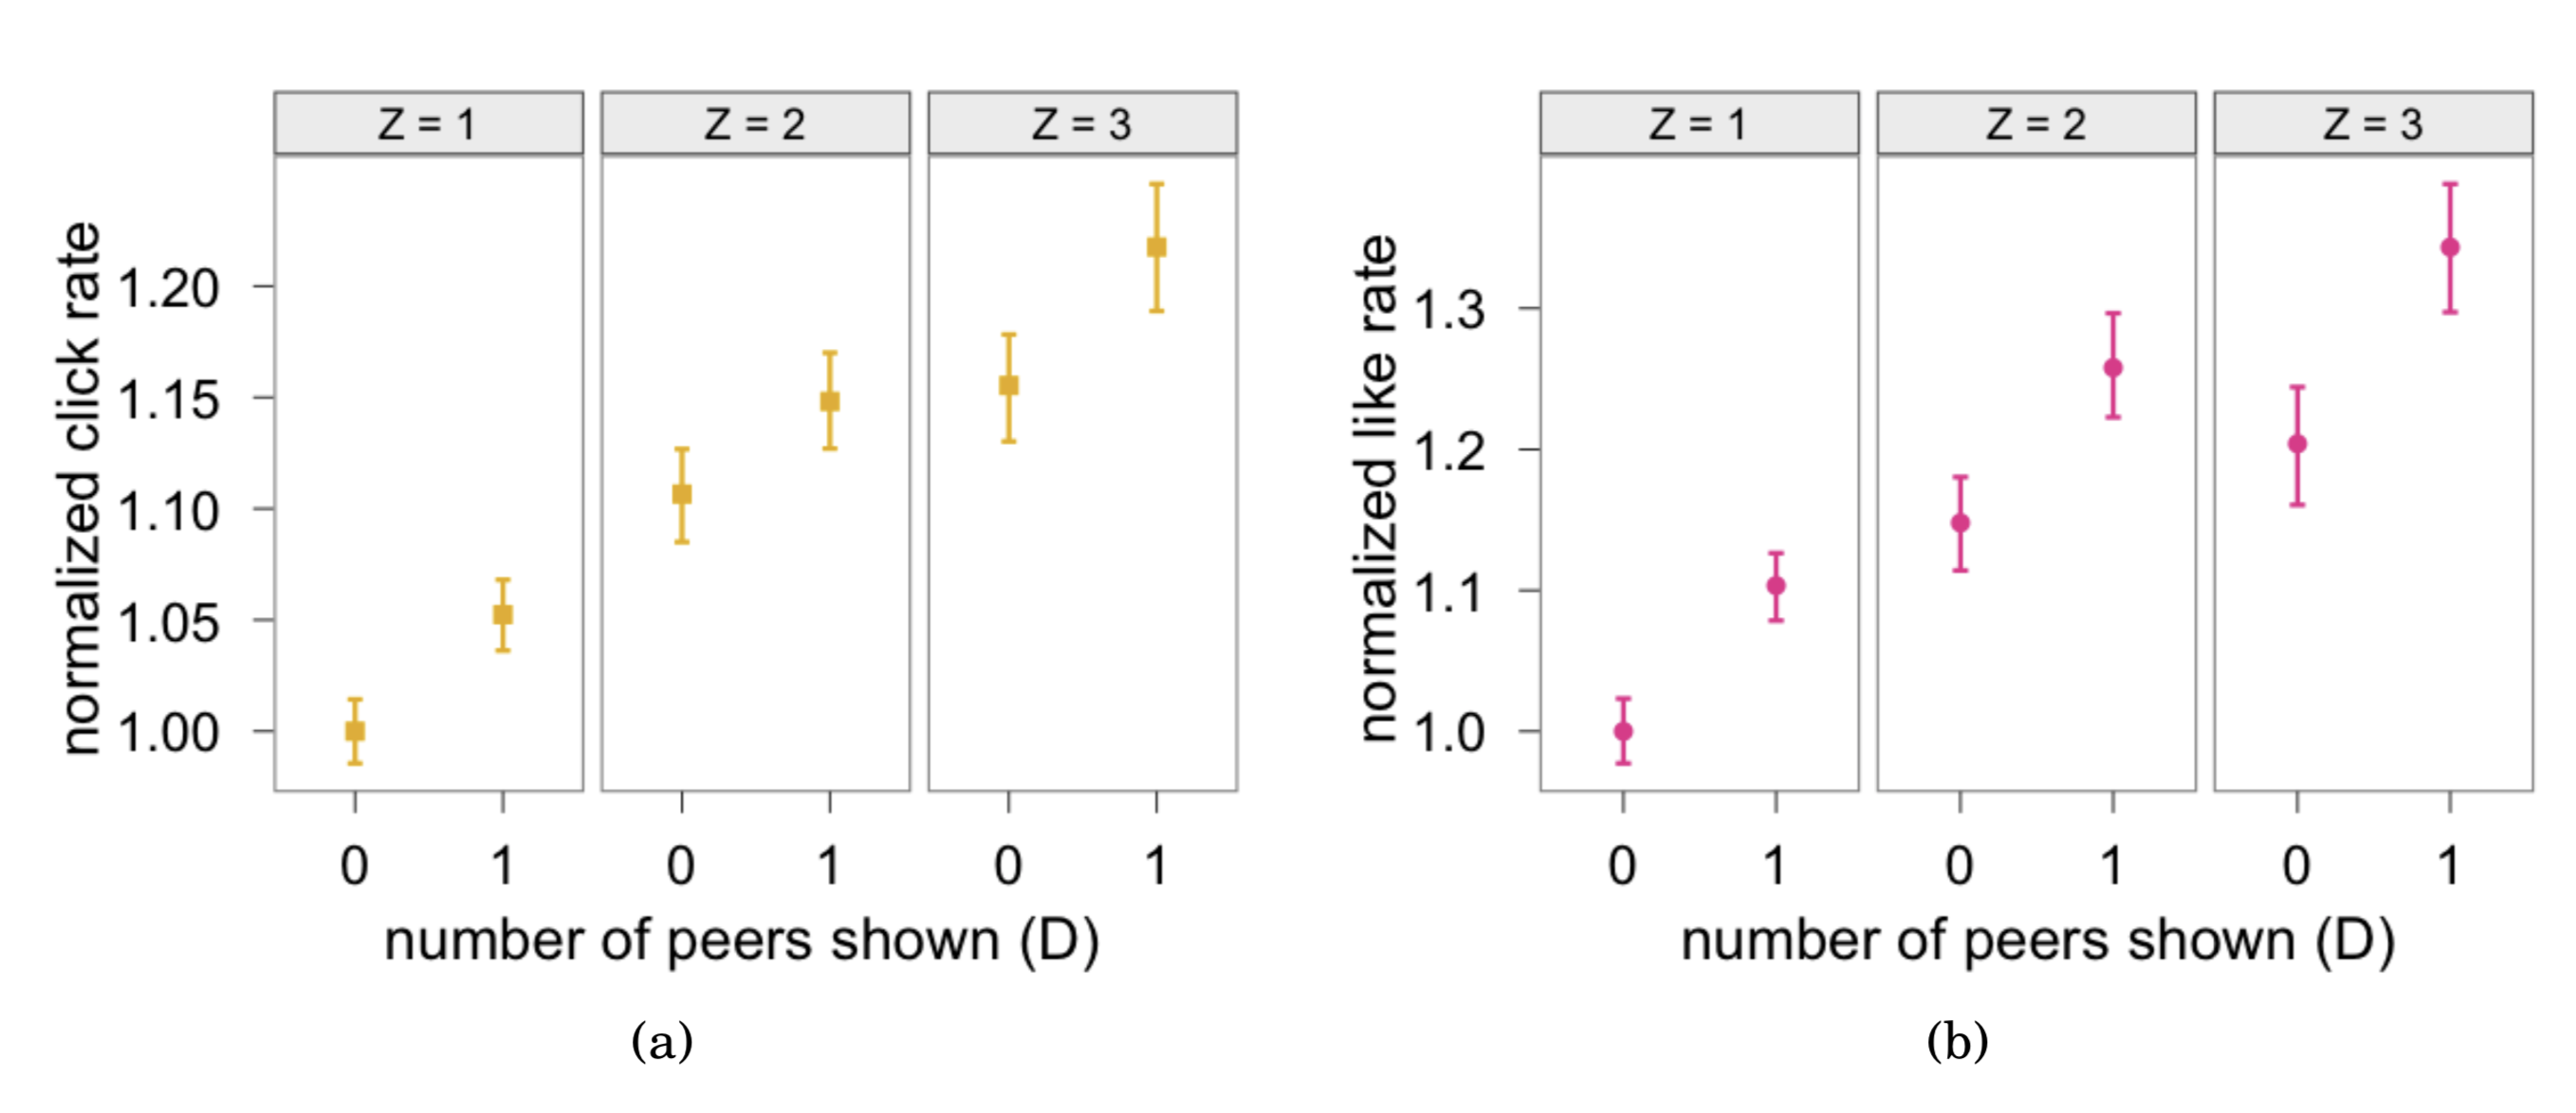
\includegraphics[width=\textwidth]{figures/bakshy_social_2012_fig5}
\end{center}

\vfill
\begin{itemize}
\item For each value of $Z$, showing specific peer leads to more clicks and likes
\item Difference between $D=0$ for different values of $Z$ suggests homophily on unobservable characteristics (but with caution)
\end{itemize}


\note{
Consistency across two metrics is good to see
}

\end{frame}
%%%%%%%%%%%%%%%%%
\begin{frame}

What about tie strength?  Who is the best person to mention to maximize click-through rates?

Tie strength between $i$ and $j$ is measured the fraction of $i$'s communication that is directed at $j$ or posts by $j$.

\end{frame}
%%%%%%%%%%%%%%%%%
\begin{frame}

\begin{center}
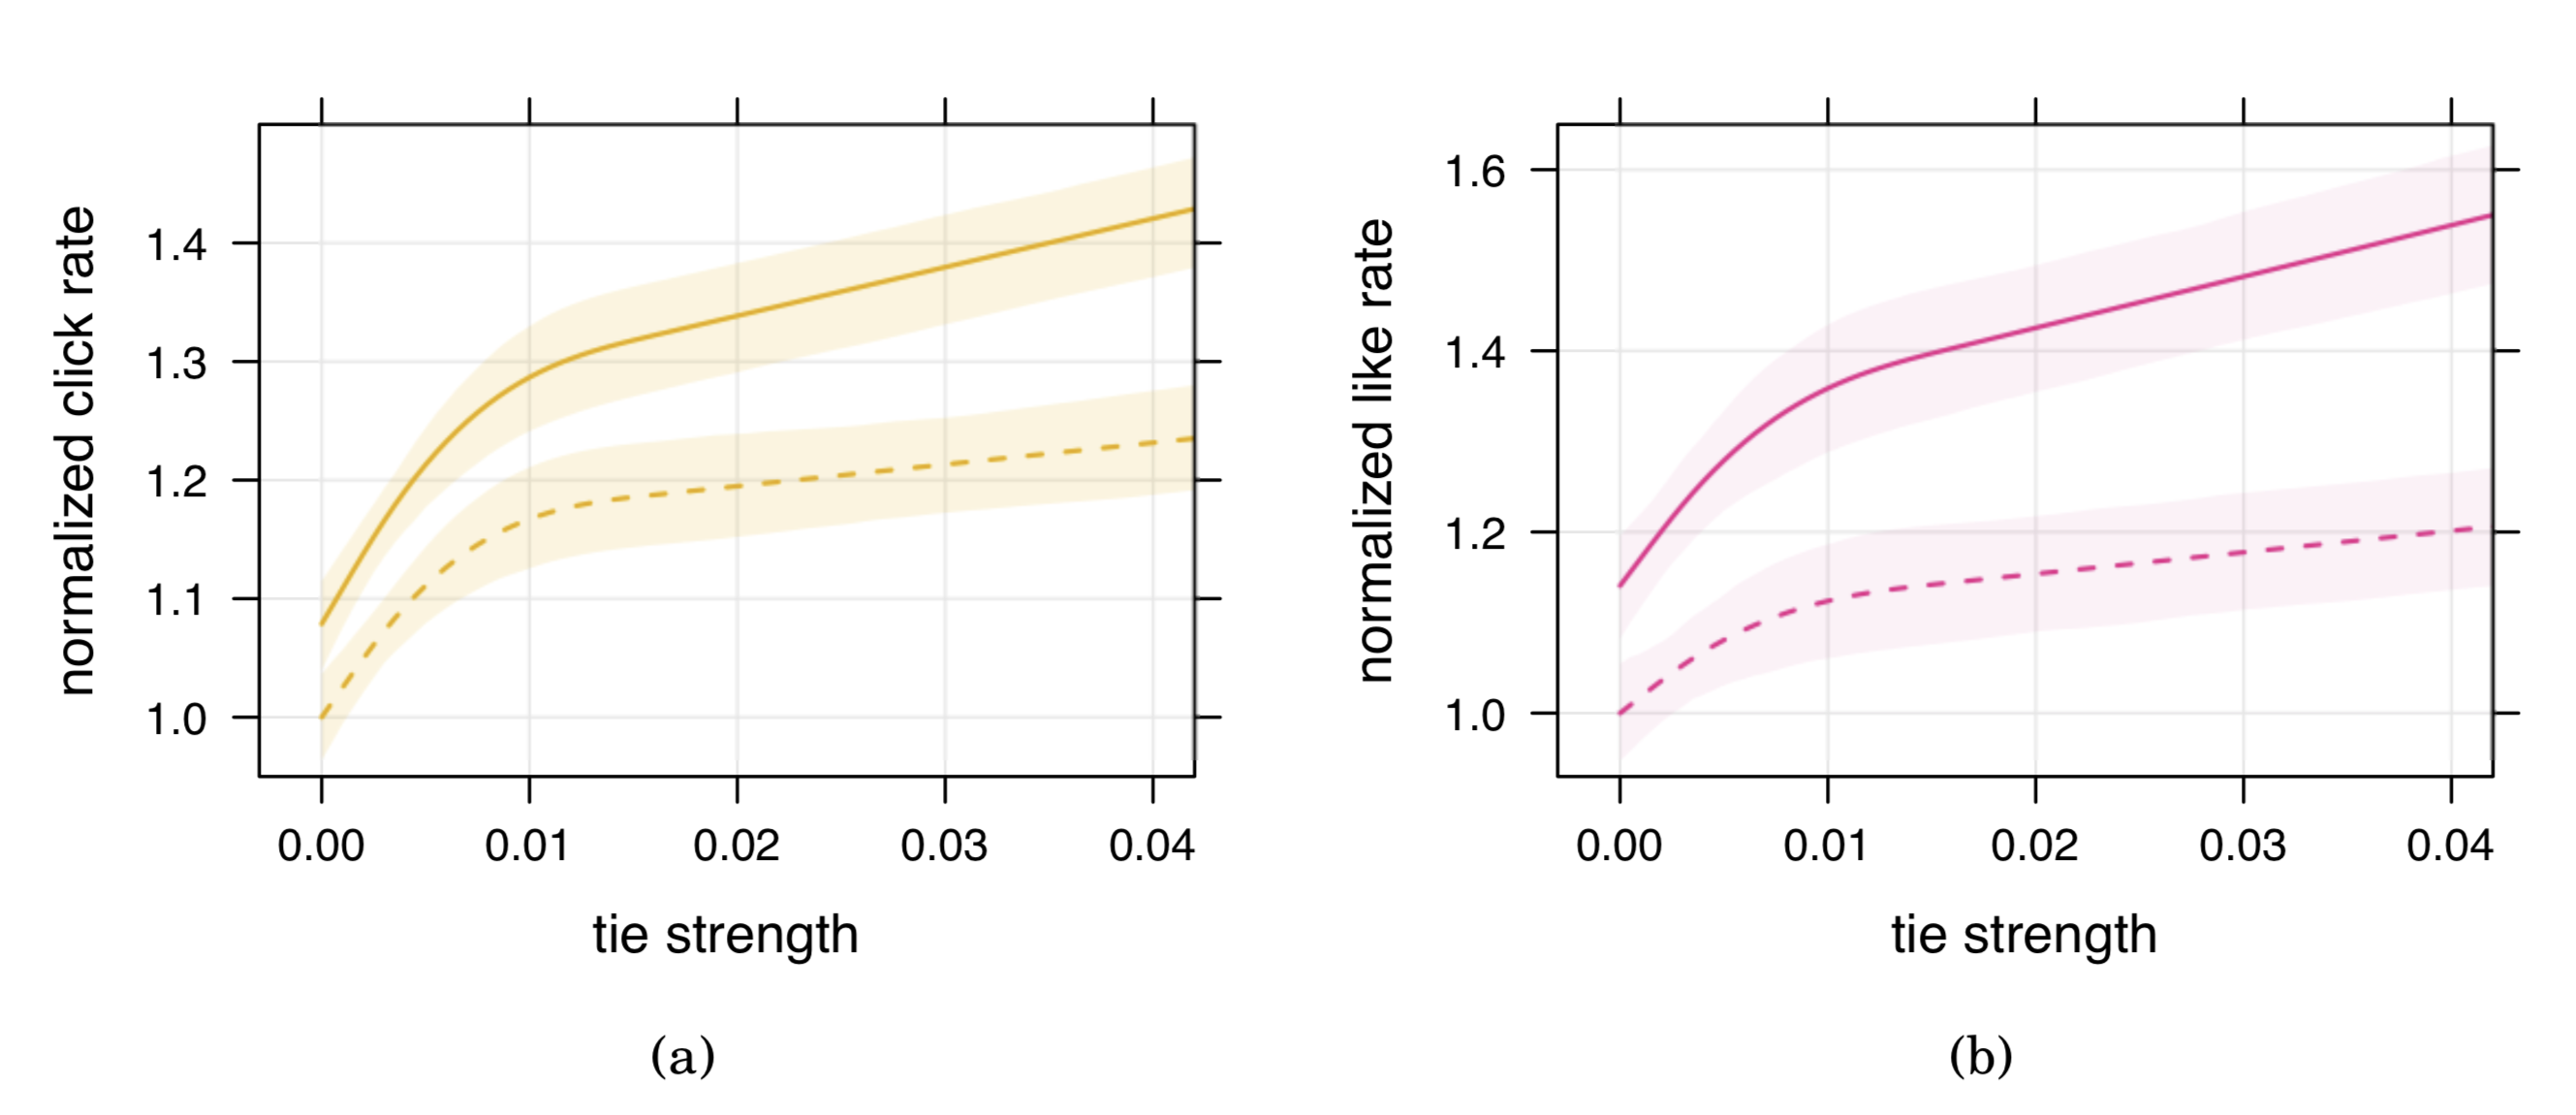
\includegraphics[width=\textwidth]{figures/bakshy_social_2012_fig7}
\end{center}

\vfill
\begin{itemize}
\item As tie strength increases, click and like rate increase whether the signal is present (solid) or absent (dashed). The risk ratio increased as tie strength increased (Fig 8).
\end{itemize}

You can bet that this information was used to decide which friend to show in the ad
\end{frame}
%%%%%%%%%%%%%%%%%
\begin{frame}

\begin{center}
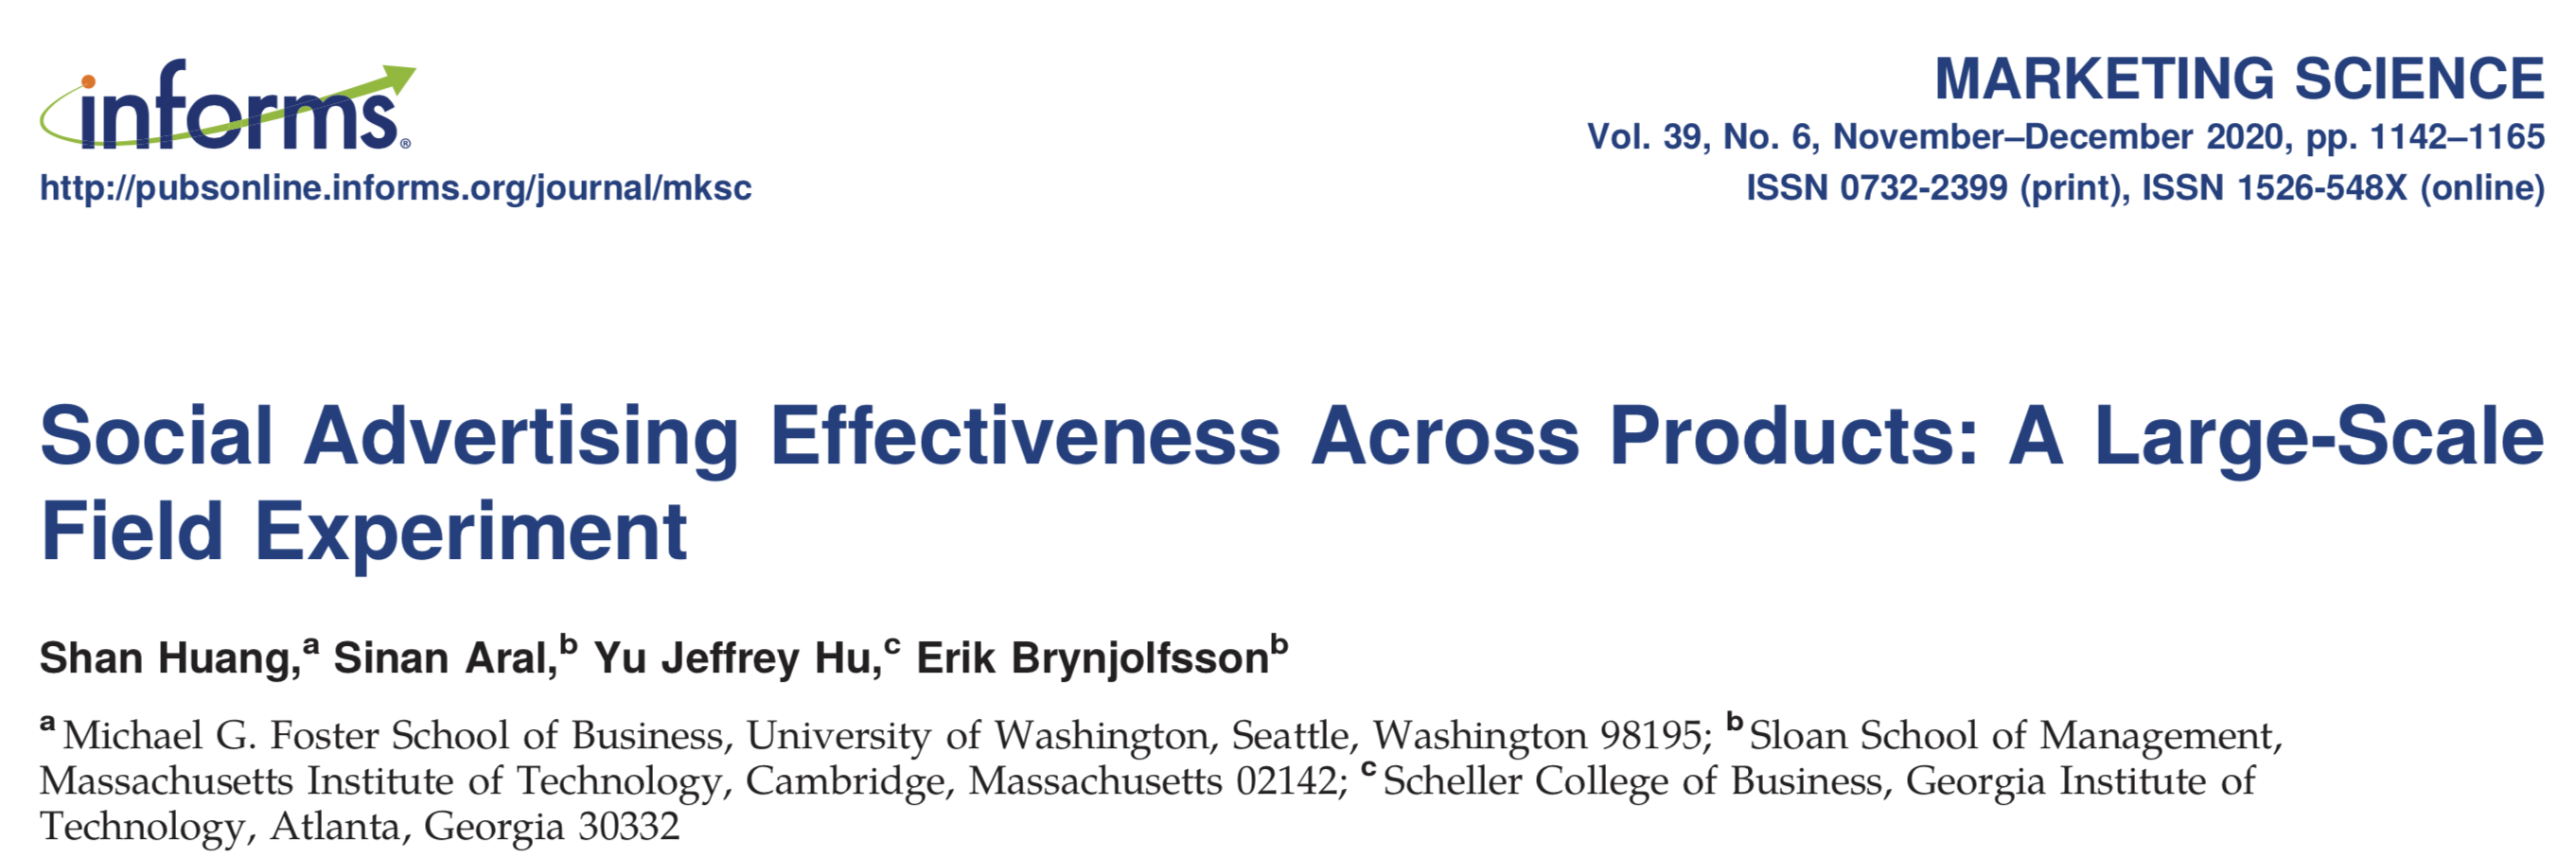
\includegraphics[width=\textwidth]{figures/huang_social_2020_title}
\end{center}

\vfill
\begin{itemize}
\item Replicate and extend Baskhy et al.\ on WeChat
\item 71 products, 25 categories, 37 million users
\end{itemize}

\end{frame}
%%%%%%%%%%%%%%%%%
\begin{frame}

\begin{center}
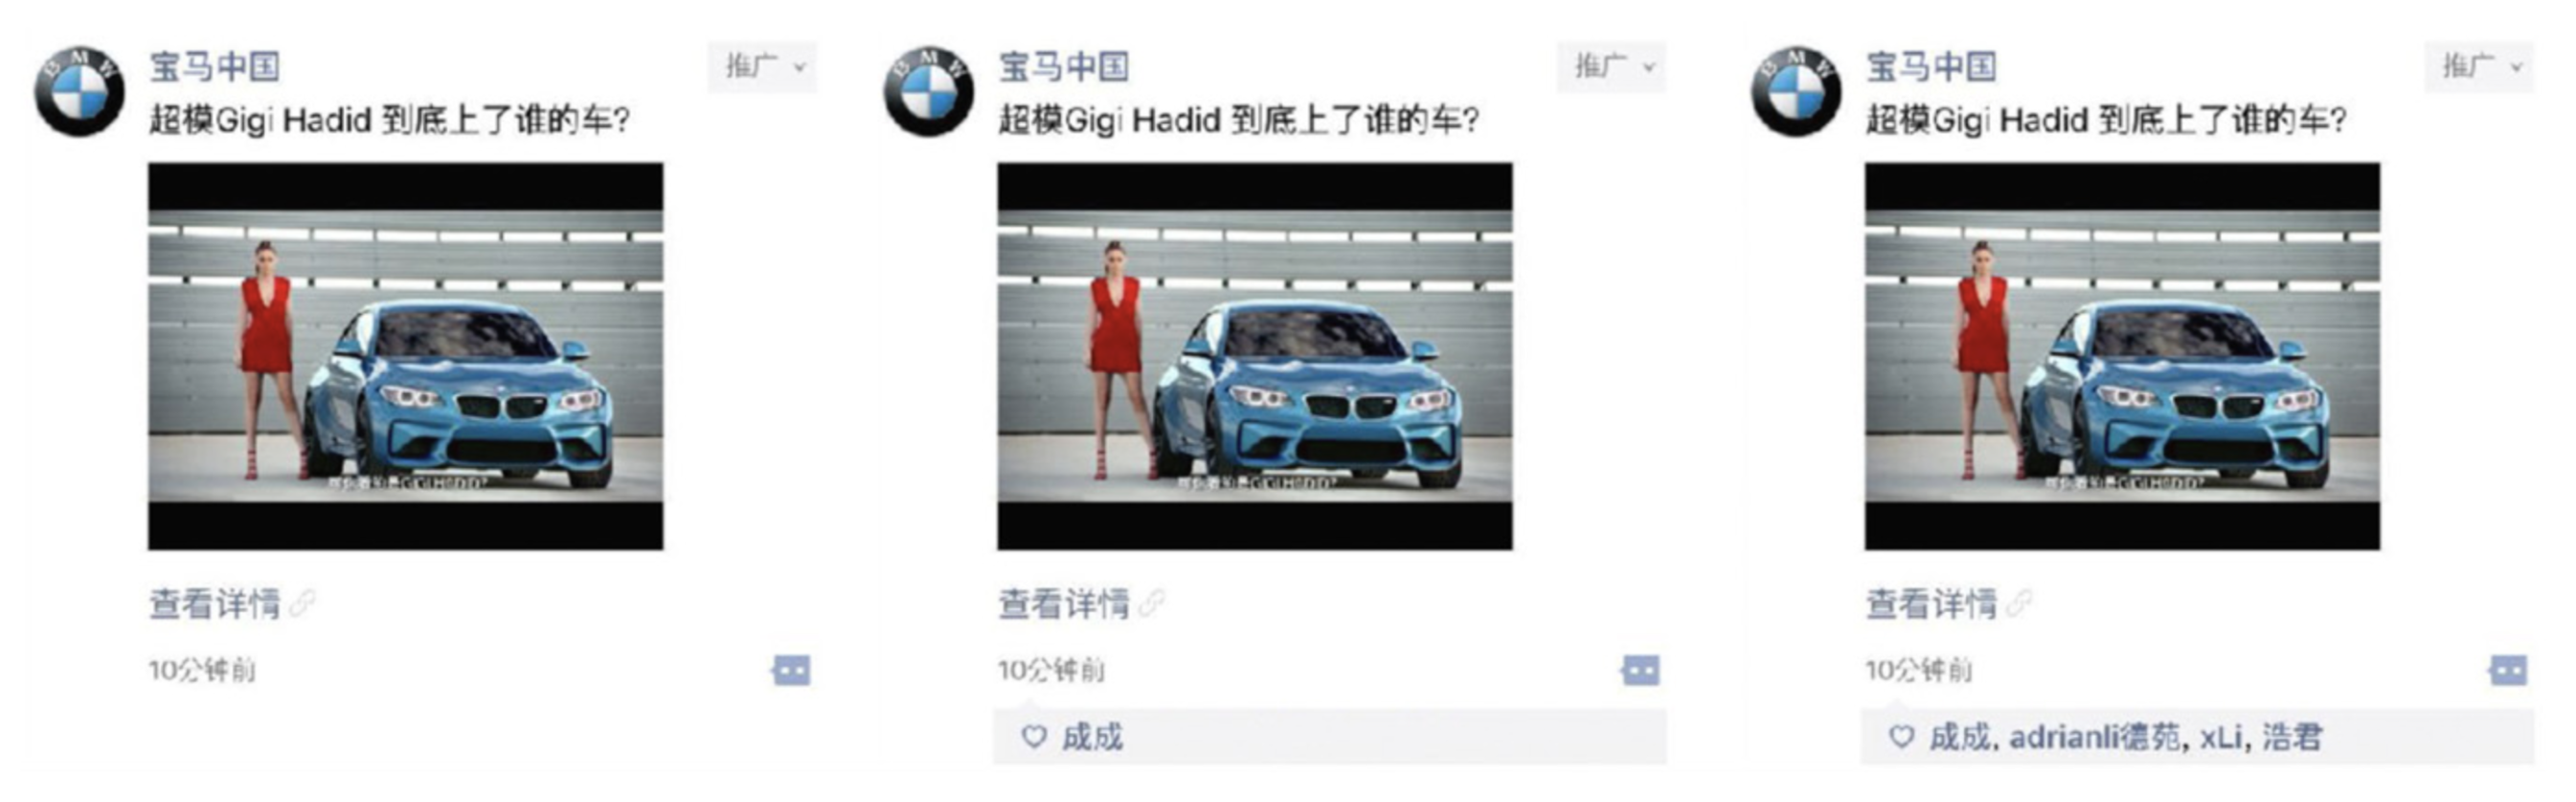
\includegraphics[width=\textwidth]{figures/huang_social_2020_fig2}
\end{center}

\begin{itemize}
\item 3 treatments: no social cue, one like, organic likes \pause
\item main comparison is between no social cue and one like \pause
\item displaying a social cue make users 33.75\% more likely to click on an ad
\end{itemize}

\end{frame}
%%%%%%%%%%%%%%%%%%%%%%%
\begin{frame}

\begin{center}
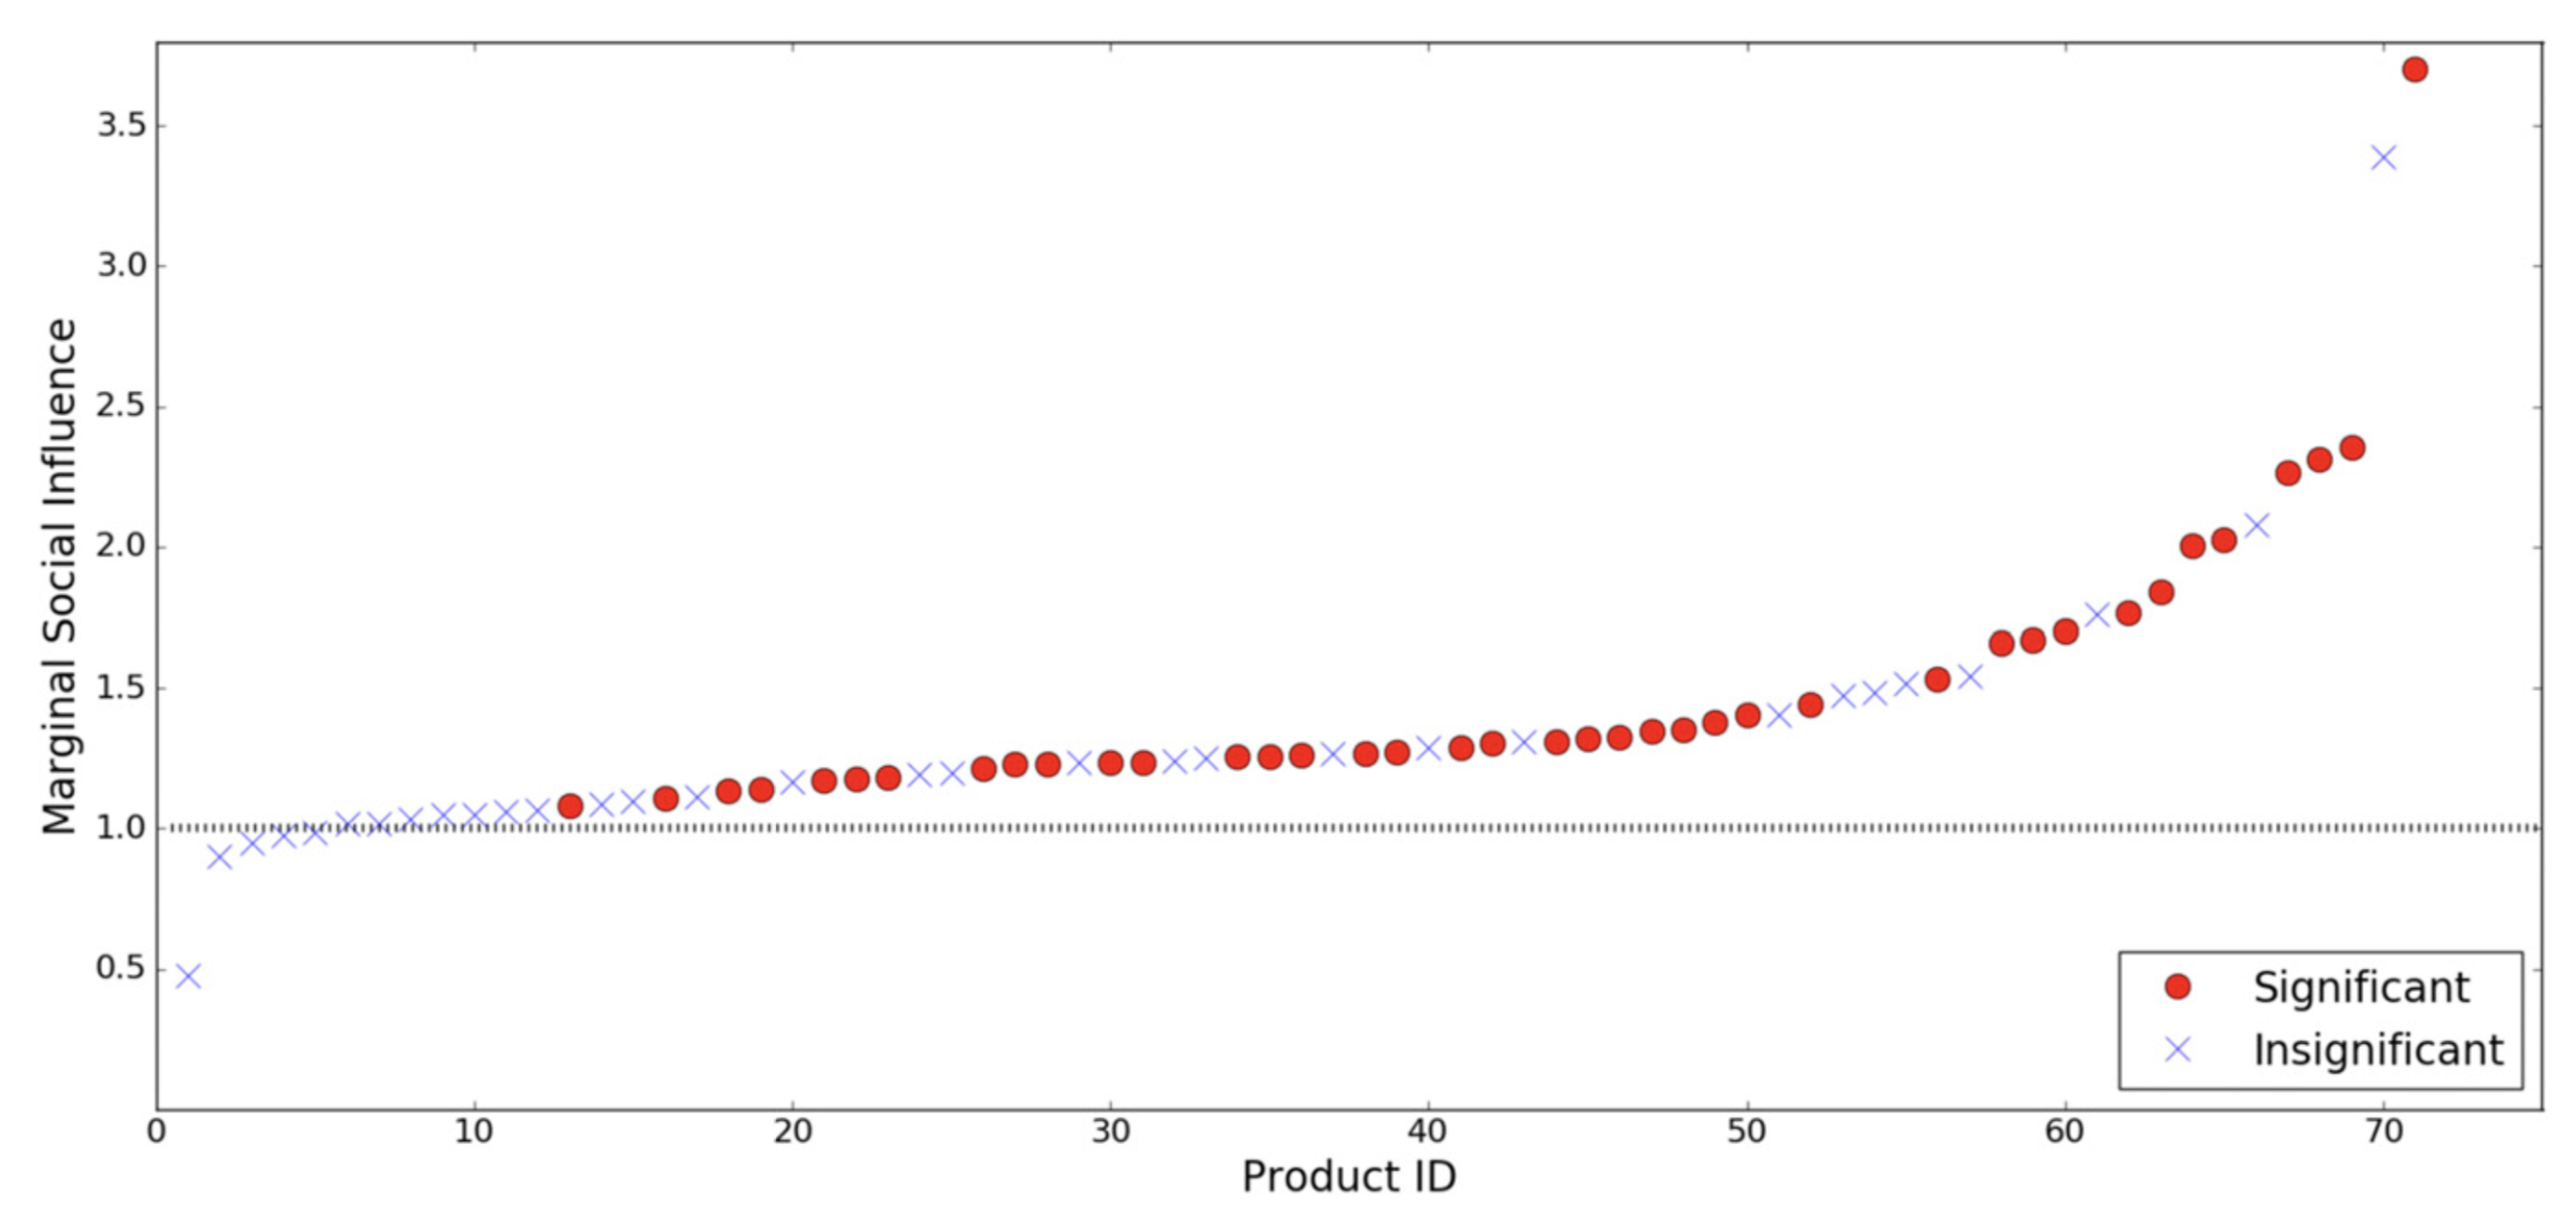
\includegraphics[width=\textwidth]{figures/huang_social_2020_fig3}
\end{center}

\begin{itemize}
\item Effect was positive for virtually all 71 products
\end{itemize}

\end{frame}
%%%%%%%%%%%%%%%%%%%%%%%
\begin{frame}

\begin{center}
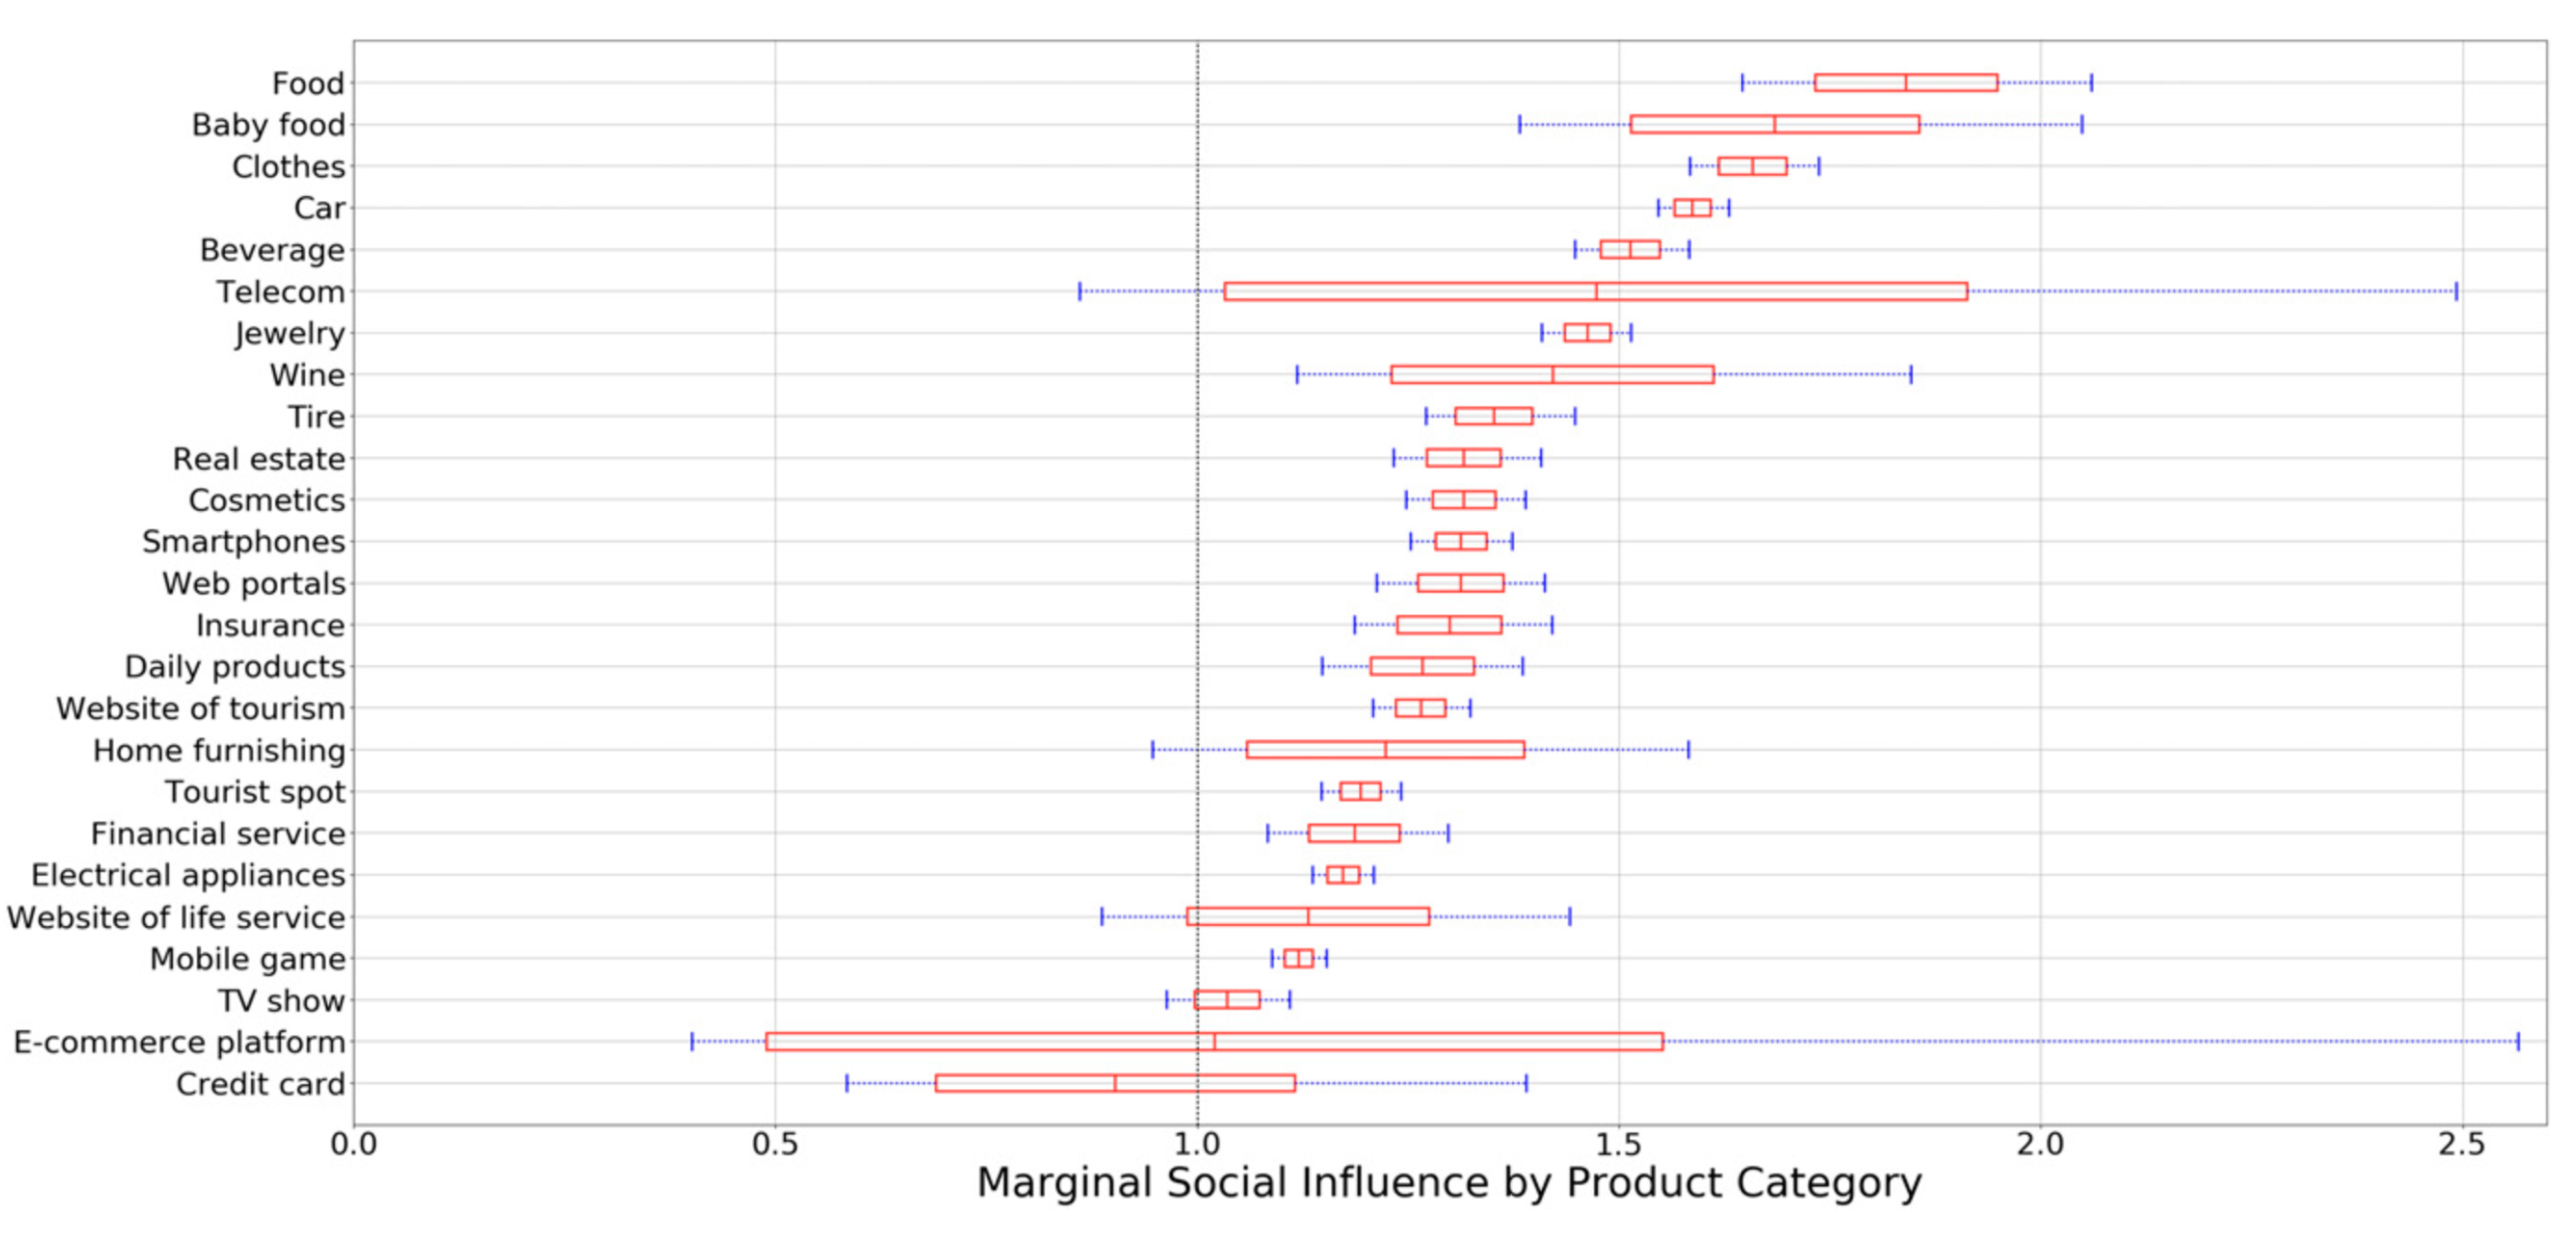
\includegraphics[width=\textwidth]{figures/huang_social_2020_fig4}
\end{center}

\begin{itemize}
\item Effect was biggest for food, baby food, clothes, and cars.
\item Effect was smallest for credit card, e-commerce platform, and a TV show
\end{itemize}

\end{frame}
%%%%%%%%%%%%%%%%%%%%%%%
\begin{frame}

Conclusions:
\begin{itemize}
\item social media enable social advertising \pause
\item network data can be used to target ads. The value of adding network data depends on the type of information the advertiser already has.  In some cases, social helped in other cases it does not.  \pause
\item network data can also be used as part of the ad itself, and social signals of different kinds can increase engagement (click-through-rate, likes)
\end{itemize}

\end{frame}
%%%%%%%%%%%%%%%%%
\begin{frame}

Fixing social media:
\begin{itemize}
\item Frank, R.H. (2021). The economic case for regulating social media. \textit{New York Times}.
\item Pennycook, G. and Rand, D. (2020). The right way to fight fake news. \textit{New York Times}.
\item Bail, C.A. et al. (2018). Exposure to opposing views on social media can increase political polarization. \textit{PNAS}.
\item Kaiser, B. et al. (2021). Adapting security warnings to counter online disinformation. \textit{30th USENIX Security Symposium (USENIX Security 21)}.
\end{itemize}

\end{frame}
%%%%%%%%%%%%%%%%%

\end{document}
